\documentclass[output=paper]{langscibook}
\ChapterDOI{10.5281/zenodo.18845928}
\author{Maria-José Ezeizabarrena\orcid{}\affiliation{University of the Basque Country (UPV/EHU), Spain, ELEBILAB Research group} and Amaia Munarriz-Ibarrola\orcid{}\affiliation{University of the Basque Country (UPV/EHU), Spain, ELEBILAB Research group} and Varun D. C. Arrazola\orcid{}\affiliation{CNRS-IKER (UMR 5478), France}}
\title[Cued GAS and L1 effects in the acceptance of mixed Basque-Spanish DPs]{Cued gender assignment strategies and L1 effects in the acceptance of mixed Basque-Spanish DPs}
\abstract{Research on mixed determiner phrases (DPs) combining languages with and without gender distinctions has highlighted the existence of individual variation in gender assignment strategies (GAS). For example, ungendered Basque nouns require the assignment of masculine or feminine gender when combined with a Spanish determiner in Basque-Spanish mixed DPs.

This chapter investigates which GAS (phonological, analogical or default) drive the acceptability of such mixed DPs. Additionally, it explores whether the bilingual profile —Spanish-dominant (L1S) versus Basque-dominant (L2S)— influences these preferences. Twenty-two early bilinguals (11 L1S, 11 L2S) with high proficiency in Basque and Spanish completed an acceptability judgment task, in which they rated 40 experimental sentences containing mixed DPs that were controlled for analogical and phonological gender.

Participants generally accepted mixed DPs, although responses indicated an interplay between analogical and phonological cues, with highest ratings for double‑match items and lowest for non‑matching ones. L1S bilinguals showed stronger rejection of non‑matching DPs, whereas L2S speakers exhibited more uniform ratings. Only in the non‑matching condition did some L1S participants show a slight preference for feminine determiners. These findings indicate that gender assignment in Basque–Spanish mixed DPs is guided by cue‑based strategies rather than default strategies, with bilingual profile shaping the relative weight of each cue.}
\IfFileExists{../localcommands.tex}{
  \addbibresource{../localbibliography.bib}
  \usepackage{tabularx,multicol}
\usepackage{url}
\urlstyle{same}

 
\usepackage{langsci-optional}
\usepackage{langsci-lgr}
\usepackage{langsci-gb4e}

\usepackage{multirow}
\usepackage{cleveref}
\usepackage{subfigure}
\usepackage{langsci-branding}

  \input{../localcommands} 
  \input{../localhyphenation} 
  \togglepaper[4]%%chapternumber
}{}

\begin{document}
\maketitle 
%\shorttitlerunninghead{}%%use this for an abridged title in the page headers

\section{Introduction }\label{sec:ezeiza:1}

Alternating between unilingual discourse in either two (or more) languages and bilingual discourse, which includes elements of more than one language, is a common praxis in many bilinguals’ daily life, {especially when interacting with interlocutors of similar linguistic backgrounds} {(\citealt{BullockToribio2009})}{. This switching from one language to another in discourse has received different names such as} {\textit{code switching}} {(henceforth CS),} {\textit{code mixing}}, {\textit{code alternation}}{, etc. The view on CS is changing in recent times and moving from being considered as an indication of (many) bilinguals’ incapacity to maintain unilingual speech, to a communicative resource that only bilinguals can benefit from, and use mostly voluntarily, in spontaneous conversation. CS can be manipulated, that is, “inhibited”, “controlled”, “forced” or “judged”, as has been shown across studies designed specifically to test bilinguals’ behaviour and/or attitudes towards CS. Thus, psycholinguistic research has provided relevant findings related to the processes involved in, for example, free switching, as compared to involuntary switching produced under cued instructions in experimental settings. Although some authors consider that “these studies together underscore the importance of understanding CS speech, as well as the implications of CS speech for bilingual language representations”} {(\citealt{XuEtAl2021}: 2)}{, it has been found that processing natural CS and artificial CS require different brain areas, and that unlike involuntary CS, voluntary CS does not necessarily incur a switching cost} {\citep{Blanco-ElorrietaEtAl2018}}.

 {Individual variation in CS has been widely attested, which confirms that not all bilinguals are producers of CS in a similar way, with the same frequency, or in the same communicative situations. For instance, the same speaker may code-switch more frequently when interacting with regular CS producers than with interlocutors who are not, whilst (s)he may not code-switch at all in conversations with interlocutors, monolinguals or not, who regularly communicate in unilingual speech or have negative attitudes towards CS} (\citealt{BlokzijlEtAl2017, Lipski2016,ParafitaCoutoEtAl2015welsh}).

{A growing body of literature recognizes the importance of studying the linguistic restrictions involved in phrases containing elements with different (lexical, grammatical, phonological) features in the corresponding languages they come from. Under the belief that the so called “conflict sites”} {(\citealt{PoplackMeechan1998})} {can provide relevant evidence for the study of the architecture of mixed utterances from a linguistic perspective, the mixed determiner phrase (DP) is the syntactic structure that has drawn the attention of most CS researchers, coming from very different theoretical and methodological approaches, and which has offered the most relevant findings on the regularities and patterns existing in both child and} {adult CS production} {(\citealt{Beatty-MartínezDussias2019,CantoneMüller2008,Chan2008,JorschickEtAl2011,LicerasEtAl2008})}. In these studies, special attention has been paid, for example, to mixed DPs involving languages that differ in word order or in a particular feature such as gender (e.g. one language without vs. another with two to three M(asculine)/F(eminine)/Neuter gender distinctions). For an updated overview on theoretical and methodological issues in CS studies see \citet{Munarriz-IbarrolaEtAl2018} {and \citet{ParafitaCoutoEtAlinpress}}.

{However, CS can be investigated at the receptive level as well. Exposure to both unilingual and mixed discourse is a common experience for many individuals living in bilingual communities. Similarly to what has been reported in production studies, individual variation has been observed in the degree of exposure to CS, as well as in the degree of acceptance} {(\citealt{Lipski2016,ParafitaCoutoEtAl2015welsh})}{. Thus, the (passive and/or active) use of CS can be considered a component of the linguistic competence of individuals, bilingual or not, living in bilingual communities. Moreover, as a feature that may allow identification of language dominance} {(\citealt{HerediaAltarriba2001})}, CS has become a phenomenon of interest in socio- and psycholinguistics. Therefore, it is worth studying the linguistic (e.g. typological distance between the languages involved), the psycholinguistic (participants’ profile, age of acquisition) as well as the sociolinguistic factors (community type, socio-economic status, prestige) affecting CS use. See \citet{Beatty-MartínezDussias2019,BlokzijlEtAl2017} and \citet{ParafitaCoutoGullberg2019}.

{In this regard, research on mixed determiner phrases (DP) has provided a fruitful literature on bilinguals’ tendencies and strategies in the configuration of such structures, as well as on the assignment or reassignment of gender features to (un)gendered nouns inserted in DP phrases containing a gender specified determiner from the other language} {\citep{BellamyParafitaCouto2022}}{. For instance, English-Spanish mixed DPs may result from the combination of a Spanish determiner (Det}{\textsubscript{S}}{) and an English noun (N}{\textsubscript{E}}{) such as in \REF{ex:ezeiza:1a}, or of an English determiner (Det}{\textsubscript{E}}{) and a Spanish noun (N}{\textsubscript{S}}{) \REF{ex:ezeiza:1b}. The expressive and receptive use of mixed DPs requires that the bilingual speaker “decides” on the language that will provide each lexical element in the mixed structure. Although theoretically both options are possible, there is robust evidence coming from early and adult spontaneous production, as well as from acceptability judgment tasks, which has demonstrated that in many different communities Det}{\textsubscript{S}}{N}{\textsubscript{E}} {mixed DPs \REF{ex:ezeiza:1a} are more frequent than the reverse Det}{\textsubscript{E}}{N}{\textsubscript{S}} {\REF{ex:ezeiza:1b}} {(\citealt{HerringEtAl2010,JakeEtAl2002,LicerasEtAl2008,MoroQuintanilla2014,ParafitaCoutoEtAlinpress,ValdésKroff2016})}.

\ea\label{ex:ezeiza:1}
\ea\label{ex:ezeiza:1a}
 la/el   house

 {the}{\textsubscript{S.F}}{/the}{\textsubscript{S.M} }{house}{\textsubscript{ E. ungendered}}

 {‘the house’}

\ex\label{ex:ezeiza:1b}
{ the   casa}

 {the}{\textsubscript{ E.ungendered}} {house}{\textsubscript{S.F}}

 {‘the house’}

\z
\z

{Option \REF{ex:ezeiza:1a} requires an additional adjustment in gender features between the lexical insertion of the N}{\textsubscript{E}} {\textit{house}} {and the Det}{\textsubscript{S}} {\textit{la/el}}{, which according to the Spanish grammar agrees in gender and number features with the lexical category that it determines. Thus, in order to evaluate the acceptance of the Det}{\textsubscript{S}} {the bilingual speaker needs to decide whether to attribute M or F gender to the (originally) ungendered N}{\textsubscript{E}} {\textit{house}}.

{The aim of this study is to gain further understanding of bilinguals’ gender assignment strategies (GAS) in mixed DPs by providing new acceptability data of mixed Basque-Spanish DP structures by two groups of bilinguals, who are regular and highly functional users of these two languages: S(panish) a gendered language, and B(asque), a non-gendered language. Similarly to English-Spanish bilinguals, Basque-Spanish bilinguals need to assign some gender value to each Basque noun (N}{\textsubscript{B}}{) inserted in mixed DPs containing a Det}{\textsubscript{S}} {\REF{ex:ezeiza:2}.}

\ea\label{ex:ezeiza:2}
\ea\label{ex:ezeiza:2a}
{ la  etxe}

 {the}{\textsubscript{S.F}} {house}{\textsubscript{ B.ungendered}} {(Spanish: ‘casa’}{\textsubscript{F}})

 {\textsubscript{} }{‘the house’}

\ex\label{ex:ezeiza:2b}
 { el   etxe}{\textsubscript{} }

 {the}{\textsubscript{S.M}} {house}{\textsubscript{ B.ungendered}} {(Spanish: ‘casa’}{\textsubscript{F}})

 {\textsubscript{} }{‘the house’}

\z
\z

{To that aim, the remaining part of the chapter proceeds as follows. \sectref{sec:ezeiza:2} deals with unilingual and mixed DPs in Basque and Spanish (\sectref{sec:ezeiza:2.1}) and gives a brief overview of the main gender assignment strategies (GAS) reported in the literature on mixed DPs predominantly in Spanish and Basque (\sectref{sec:ezeiza:2.2}). After presenting the aims and research questions (\sectref{sec:ezeiza:2.3}), in section 3 we present the methodological details of the study: participants (\sectref{sec:ezeiza:3.1}), procedure} (\sectref{sec:ezeiza:3.2}), materials (\sectref{sec:ezeiza:3.3}) and predictions {(\sectref{sec:ezeiza:3.4}). \sectref{sec:ezeiza:4} analyses the results, which are discussed in \sectref{sec:ezeiza:5}.}

\section{Gender assignment}\label{sec:ezeiza:2}

In general, (monolingual and bilingual) Spanish speakers know that some nouns like \textit{cañón} ‘canyon’ and \textit{mapa} ‘map’ are M(asculine), whereas \textit{acción} ‘action’, \textit{canción} ‘song’, \textit{hierba} ‘grass’ or \textit{mano} ‘hand’ are F(eminine). The knowledge of the morphosyntactic, phonological and semantic properties of N\textsubscript{S} allows speakers to combine each of them with the corresponding M/F determiner –\textit{el} ‘the\textsubscript{M}’, \textit{un} ‘a\textsubscript{M}’, \textit{este} ‘this\textsubscript{M}’ or \textit{la} ‘the\textsubscript{F}’, \textit{una} ‘a\textsubscript{F}’, \textit{esta} ‘this\textsubscript{F}’– in unilingual Spanish DPs (\citealt{Corbett2006,Roca2005}).

Each N\textsubscript{S} has its gender specificity, which is (highly) predictable through noun endings, and less idiosyncratic than in other languages such as French or German. For instance, virtually all N\textsubscript{S} ending in \textit{{}-o} are M (99.87\%) and the majority of the N\textsubscript{S} ending in \textit{{}-a} (96.30\%) are F (\citealt{Eddington2002,TeschnerRussell1984}).

However, not all noun endings in this language are so “informative”, and hence the distinction between the so-called “regular”, “canonical” or “transparent” nouns (5-6) –M nouns ending in \textit{-o} and F nouns ending in \textit{-a} –  as opposed to “irregular”, “non-canonical” or “opaque” nouns (3-4) (\citealt{CaffarraBarber2015,ViglioccoEtAl1997}). Note that apart from \textit{-a} and \textit{-o} endings, most of other endings tend to appear in M nouns, since only 6.93\% of \textit{-i} ending, 4.9\% of \textit{-u} ending, 10.65\% of \textit{-e} ending and 51.6\% of \textit{-n} ending N\textsubscript{S}are F.

\ea%3
    \label{ex:ezeiza:3}
     \ea el   estuche\\
         the\textsubscript{M}  case\textsubscript{M}            \\
    ‘the pencil case’
    \ex la   clase\\
     the\textsubscript{F}  classroom\textsubscript{F}\\
     ‘the classroom’
    \z
\z

\ea%4
    \label{ex:ezeiza:4}
    \ea la   mano                                          \\
         the\textsubscript{F}  hand\textsubscript{F}         \\
         \glt ‘the hand’

     \ex
     \gll el   pijama     \\
      the\textsubscript{M}  pyjama\textsubscript{M}     \\
     \glt ‘the pyjama’
    \z
\z

{Spanish grammar requires that (monolingual and bilingual) speakers “attribute” one of the two gender values available in Spanish, M or F, to the inserted noun, which will determine further combinations of the} {noun with many other gender-inflected words such as determiners (3-4), quantifiers (}{\textit{algun/a}} {‘some’}{\textit{; poco/a}} {‘(a) few’), and adjectives (}{\textit{blanco/a} } {‘white’), as well as the gender marking of other phrasal elements such as pronouns and copula-constructions.}

{The specificities of the languages involved in a mixed DP may affect bilinguals’ decisions regarding gender assignment to the inserted noun differently, depending on whether both languages distinguish gender (e.g, Italian and Spanish distinguishing M/F; or Sp (M/F)-German (M/F/Neuter)) or whether only one language distinguishes gender (e.g. Spanish M/F-English, Spanish-Papiamento or Spanish-Basque). See} \sectref{sec:ezeiza:2.2} and \citet{BellamyParafitaCouto2022} {for more details on the patterns found across language dyad combinations and code-switcher profiles.}

\subsection{Unilingual and mixed DPs in Basque and in Spanish}\label{sec:ezeiza:2.1}

Basque is a language without gender marking and, consequently, the M/F opposition found in many lexical pairs in Spanish, related \REF{ex:ezeiza:5a}-\REF{ex:ezeiza:5b} or not related to biological sex \REF{ex:ezeiza:6a}-\REF{ex:ezeiza:6b}, is realized in Basque as differentiated lexical items \REF{ex:ezeiza:5c}-\REF{ex:ezeiza:5d}, \REF{ex:ezeiza:6c}-\REF{ex:ezeiza:6d}.

\ea\label{ex:ezeiza:5}
  \ea\label{ex:ezeiza:5a}
    niñ-o\\
    child-M\\
    \glt ‘boy’
  \ex\label{ex:ezeiza:5b}
    niñ-a\\
    child-F\\
    \glt ‘girl’
  \ex\label{ex:ezeiza:5c}
    mutil\\
    \glt ‘boy’
  \ex\label{ex:ezeiza:5d}
    neska\\
    \glt ‘girl’
  \z
\z


\ea\label{ex:ezeiza:6}
  \ea\label{ex:ezeiza:6a}
    \gll cerez-o\\
         cherry-M\\
    \glt ‘cherry’
  \ex\label{ex:ezeiza:6b}
    \gll cerez-a\\
         cherry-F\\
    \glt ‘cherry’
  \ex\label{ex:ezeiza:6c}
    gerezi-ondo\\
    \glt ‘cherry-tree’
  \ex\label{ex:ezeiza:6d}
    gerezi\\
    \glt ‘cherry (fruit)’
  \z
\z

{The existence / absence of grammatical gender has consequences in the features of DPs in both languages, which differ in a set of additional morphosyntactic features} {\citep{Corbett2006}}{. First, determiners and quantifiers always precede nominal elements in Spanish \REF{ex:ezeiza:7a}-\REF{ex:ezeiza:7c}, whereas variation in placement is attested in Basque, where the determiner may be the suffixed article –}{\textit{a}} (\ref{ex:ezeiza:8}a, b), a free word which {follows the noun (demonstrative in \REF{ex:ezeiza:8c}) or a free morpheme preceding it (numerals \REF{ex:ezeiza:8c}). Second, determiners, quantifiers and adjectives match in gender and number with the modified noun in Spanish (\ref{ex:ezeiza:7}a, b, c). In contrast, no DP internal agreement is found in Basque between the noun and the rest of DP components, where all DPs’ number and case markers are attached to the last word of the DP. This last word can be a noun \REF{ex:ezeiza:8a}, an adjective \REF{ex:ezeiza:8b} or a demonstrative \REF{ex:ezeiza:8c}.}

\ea\label{ex:ezeiza:7}
    \ea\label{ex:ezeiza:7a}
        la   rama\\
        the.F branch\\
        \glt ‘the branch’
\ex\label{ex:ezeiza:7b}
        las  rama-s blanc-a-s\\
        the.F-\textsc{pl} branch-\textsc{pl}  white-F-\textsc{pl}\\
        \glt‘the white branches’
\ex\label{ex:ezeiza:7c}
     aquella-s   tres  rama-s\\
     those-F-\textsc{pl}  three  branch-\textsc{pl}\\
    \glt ‘those three branches’
    \z
\z

\ea%8
    \label{ex:ezeiza:8}
\ea \label{ex:ezeiza:8a}
    adarr-a          \\
    branch-the           \\
    \glt  ‘(the) branch’

\ex \label{ex:ezeiza:8b}
    adar   txuri-a-k \\
    branch white-the-\textsc{pl} \\
\glt  ‘(the) white branches’

\ex \label{ex:ezeiza:8c}
    hiru   adar     haiek\\
    three branch those\\
 \glt   ‘those three branches’
     \z
\z

Noteworthy, \textit{-a} {ending nouns are the most common option when naming/listing objects in Basque. Thus, the expected response to the question} {\textit{Nola esaten da “branch” euskaraz?}} {‘How do you say “branch” in Basque?’ is} {\textit{adarra}} {\REF{ex:ezeiza:8a} rather than the root *}{\textit{adar}}{. Therefore, more than one phonological form can be predicted for the lexical insertion} {\textit{adar(ra)}} {‘branch’ into Spanish \REF{ex:ezeiza:9}, which could be parsed either as a mono-morphemic \REF{ex:ezeiza:9a} or as a complex word containing a lexical root plus a grammatical ending \REF{ex:ezeiza:9b}. Similarly, the N}{\textsubscript{S}} {\textit{rama}} {‘branch’ could be treated by the switcher as a single lexical unit \REF{ex:ezeiza:10a} or as a morphological complex \REF{ex:ezeiza:10b}, made up of the root} {\textit{ram}} {and the} {\textit{-a}} {ending when inserting it in a Basque sentence.}

\ea\label{ex:ezeiza:9}
\ea\label{ex:ezeiza:9a} adarra

\ex\label{ex:ezeiza:9b} adarr-a
\z
\z

\ea\label{ex:ezeiza:10}
\ea\label{ex:ezeiza:10a} rama
\ex\label{ex:ezeiza:10b} ram-a
\z
\z

Spanish grammar requires that every determiner matches in M/F features with the noun following it. Such a rule applies indistinctively to Spanish nouns, to borrowings and to lexical insertions in which Spanish is the host language. In order to fulfil the Det-N feature agreement requirements of the Spanish grammar on DPs, Basque nouns inserted in Spanish DPs undergo a morpho(phono)logical adaptation process of genderization, which consists in the attribution of M or F gender features to originally ungendered nouns \citep{Lopez2020}. Thus, a number of options are potential candidates for the producer of mixed Det\textsubscript{S}N\textsubscript{B} DPs containing a N\textsubscript{B} such as \textit{adar} ‘branch’ (\ref{ex:ezeiza:11}a-d).

\ea
\label{ex:ezeiza:11}

\ea la adar
\ex el adar
\ex la adarra
\ex el adarra
\z
\z

\subsection{Gender assignment strategies in mixed DPs}\label{sec:ezeiza:2.2}

Some studies on mixed DPs provide evidence for the {\textit{analogical criterion}} {in mixed English-Spanish DPs, in which the gender-marked Spanish article (M)asculine} {\textit{el} }{or (F)eminine} {\textit{la}}{, preceding the ungendered English N, is selected based on the gender specificity (M or F) of the Spanish translation of the English noun (see \tabref{tab:ezeiza:1}). This analogical strategy, which has been considered the “correct” gender assignment strategy (GAS) by some researchers} {\citep{JorschickEtAl2011}}{, is closely related to the term} {\textit{translation equivalent}} {(\citealt{BellamyParafitaCouto2022})}{, although some of the levels of similarity (e.g. morphological analogy) covered by} {\textit{translation equivalent}}{, are not necessarily covered by the former in CS literature. In contrast, the} {\textit{masculine default}}{, according to which speakers tend to select/prefer masculine mixed DPs, regardless of the features of the English noun inserted, is the most frequent strategy in mixed English-Spanish DPs} {(\citealt{OthegyLapidus2003})}{, especially for code-switchers who are dominant in the non-gendered language, English} {(\citealt{Beatty-MartínezDussias2019,LicerasEtAl2008,ValdésKroff2016})}{. See also \citet{BellamyParafitaCouto2022}} {for a more detailed discussion. Finally, the} {\textit{phonological criterion}} {establishes the gender value of the N according to formal properties in some languages. This may be the case for Spanish, where the fact/rule that most} {\textit{-a/-o}} {ending N}{\textsubscript{S}} {are F/M} {(\citealt{TeschnerRussell1984})} {can be extended to lexical insertions from other (gendered or ungendered) languages.}

\begin{table}
\begin{tabularx}{\textwidth}{lXXXl}
\lsptoprule
 & \multicolumn{2}{c}{{ \textbf{Spanish-English} \textbf{DPs}}} & \multicolumn{2}{c}{{ \textbf{Spanish-Basque} \textbf{DPs}}}\\
& { \textbf{Det\textsubscript{S}}\textbf{N\textsubscript{E}}} & { \textbf{Det\textsubscript{S}}\textbf{N\textsubscript{E}}} & { \textbf{Det\textsubscript{S}}\textbf{N\textsubscript{B}}} & { \textbf{Det\textsubscript{S}}\textbf{N\textsubscript{B}}}\\
\midrule
{ Analogical criterion} & { la skirt} & { el eye} & { la gona} & { el begi(a)}\\
{ Masculine default} & { el skirt} & { el eye} & { el gona} & { el begi(a)}\\
{ Feminine default} & { la skirt} & { la eye} & { la gona} & { la begi(a)}\\
{ Phonological criterion} & { el skirt} & { el eye} & { la gona} & { el begi/ la begia}\\
\lspbottomrule
\end{tabularx}
\caption{Examples of four gender assignment strategies in S-E and S-B mixed DPs.}
\label{tab:ezeiza:1}
\end{table}

Diverging GAS have also been reported for mixed Spanish-Basque DPs in acceptability judgment studies, where the \textit{masculine default} found by \citet{BadiolaSande2018} contrasts with the preference for the \textit{analogical criterion} \citep{Iriondo2017} and also with the preference for feminine attested by \citet{ParafitaCoutoEtAl2015basque}. More recently, \citet{Munarriz-IbarrolaEtAl2022} discussed the masculine default and the feminine default as hypotheses compatible with the \textit{phonological criterion} \REF{ex:ezeiza:4}. This criterion, which establishes the gender value of the Det\textsubscript{S} in mixed Spanish-Basque DPs according to the N\textsubscript{B} word ending, is compatible with the tendency to assign F to lexical insertions with \textit{-a} ending (pronounced as /a/ in production and written as “a” in acceptance tasks) and to assign M to words with \textit{-o}, other vowels and consonantal endings. Furthermore, elicitation data analyzed by \citet{Munarriz-IbarrolaEtAl2022} confirmed the existence of different GAS among bilingual users of the same language pair, in line with \citegen{BellamyEtAl2018} study on mixed Purepecha-Spanish DPs.

Interestingly, the differences in the production patterns identified among the Basque-Spanish bilinguals tested, all of them regular users of both languages, were related to the participants’ L1. That is, L1S participants, who were either successive bilinguals with Spanish as their only L1 or simultaneous bilinguals with Spanish as one of their first languages, relied on the analogical criterion rather than on the phonological one. In contrast, successive bilinguals with Basque as their only L1 (and Spanish as their L2 or L2S) often relied on the phonological ending of the word, as evidenced by their preference for F determiners preceding \textit{-a} ending nouns.

Note that \citet{BadiolaSande2018} identified two opposed gender preferences: a generalized preference for M Det \textit{el} over F Det \textit{la} with N\textsubscript{B} like \textit{bikote} ‘couple’ \textit{batzar/ batzarra} ‘meeting’; and a F preference with a specific subclass of \textit{-a} ending words such as \textit{la makila} ‘the stick’. In this subclass the \textit{-a} ending of the word matches the root ending –\textit{a}. Thus, the phonological GAS (“choose F for \textit{-a} ending roots/words, M for the rest”), seems to provide a more satisfactory explanation than the F default.

Summing up this section, gender features in Spanish are item-specific abstract values mostly associated to nouns’ lexical and formal features (animacy, word ending, a.o.), which can be overtly expressed as M/F(/Neuter) marks in N\textsubscript{s} and other categories agreeing with them (determiners, adjectives, quantifiers). Both the specific gender value (overtly expressed or not) associated with each N\textsubscript{\MakeUppercase{s}} and the Det-N agreement rule inside DPs are stable components across varieties of Spanish. There is enough evidence in the research on Spanish bilingualism consistent with the assumption that similarly to unilingual DPs, where Det\textsubscript{S} obligatorily share gender features with the N\textsubscript{S} they precede, Det\textsubscript{s} concord with the inserted N in mixed DPs. In contrast, the variation found regarding the overt gender features of mixed DPs, in and across bilingual communities, is compatible with the (co-)existence of different GAS in the use of lexical insertions, which can be modulated by speakers’ L1, input and task.

\subsection{Aims and research questions}\label{sec:ezeiza:2.3}

The current paper aims to respond to two main research questions (RQ). RQ1 is related to the gender feature assignment to novel/inserted nouns in the host language Spanish, as well as to the gender feature agreement between Det\textsubscript{S} and N\textsubscript{B} in Basque-Spanish mixed DPs. More specifically, RQ1 aims to test whether any of the four GAS (1-4) reported in previous studies prevails as the best account of the acceptance patterns of Basque-Spanish mixed DPs (Det\textsubscript{S}N\textsubscript{B}) by early bilinguals with high functionality in the use of those two languages:

\begin{enumerate}
\item Phonological GAS, according to which inanimate N\textsubscript{B}  with \textit{-a} ending are assigned F gender whilst inanimate N\textsubscript{B} with \textit{-o,} as well as most N\textsubscript{B} with \textit{-i, -e, -u, -n} and \textit{-tz} endings, are assigned  M gender.
\item Analogical GAS, according to which inanimate N\textsubscript{B} are assigned the gender feature of the Spanish translation equivalent.
\item Masculine default strategy, according to which inanimate N\textsubscript{B} tend to be assigned M gender.
\item Feminine default strategy, according to which inanimate N\textsubscript{B} tend to be assigned F gender.
 \end{enumerate}

RQ2 is whether differentiated patterns associated with bilingual profiles can be identified in acceptability tasks, in line with previous experimental studies on mixed DPs controlling for word ending and analogical gender of the inserted N\textsubscript{B}. \citet{Munarriz-IbarrolaEtAl2022} demonstrated that cued GAS rather than (M- or F-) default strategies account for the patterns found in the elicited production of mixed Basque-Spanish DPs and that GAS variation is related to bilinguals’ L1, in the sense that:

\begin{enumerate}
\item[i.]  Basque-Spanish bilinguals with Spanish as their first (L1S) and dominant language appear to be more strongly attuned to the analogical strategy than to the rest of GAS, whilst
\item[ii.] Basque-Spanish bilinguals with Spanish as second language (L2S) and Basque as their first and regularly used language follow the phonological GAS predominantly.
\end{enumerate}

\section{Method}\label{sec:ezeiza:3}

\subsection{Participants}\label{sec:ezeiza:3.1}

Twenty-three young Spanish-Basque bilinguals participated in this study. Participants that rated 4 or more of 10 quality control unilingual sentences as incorrect were excluded from the study. One participant was excluded for this reason. The final sample was based on 22 participants (mean age 26.9, SD 4.9). Participants were divided into two groups based on bilinguals’ language dominance: 11 \textit{L2 Spanish} bilinguals (L2S) and 11 \textit{L1 Spanish} bilinguals (L1S) (including both  simultaneous bilinguals (2L1) and L1 Spanish L2 Basque early sequential bilinguals (L2S)). Dominance is here understood as a function of a variety of categories such as (the language of most) exposure, and (higher) proficiency and usage, in line with \citet{Meisel2019} and \citet{Montrul2016}. Accordingly, L2S bilinguals were all early sequential bilinguals with Basque as L1 and Spanish as L2, whilst L1S bilinguals were either early sequential bilinguals with Spanish as L1 and Basque as L2 (n = 7) or bilinguals exposed to and users of the two languages, Spanish and Basque, from birth (2L1, n = 4).

As \tabref{tab:ezeiza:2} shows, most L2 participants (9 out of 11) live in sociolinguistic environments with over 50\% Basque-speaking population (n=2 / 8 / 1 participants live in sociolinguistic areas (S areas) 2/3/4 respectively), whereas most of L1 Spanish participants live in S areas with less than 50\% of Basque speakers (n=4 / 3/ 4 participants live in S areas 1, 2 and 3, respectively. See \citet{SoziolinguistikaKlusterra2014}.

Based on the information provided in the language background questionnaire \citep{Munarriz-IbarrolaEtAl2022}, all participants attended schools where Basque is the language of instruction, use both languages on a daily basis, and can be considered as highly proficient bilinguals, considering that most of them (19, 86.3\%) have obtained the highest proficiency diploma in Basque (C1 or similar according to the CEFR).

Regarding self-rated proficiency and dominance, L2S participants rated themselves higher in Basque than in Spanish, as opposed to L1S participants, who rated themselves higher in Spanish. Thus, L1 and language dominance in context and use converge in this sample, where most L1S participants have Spanish as L1 (solely or together with Basque), live in Spanish-dominant areas and reported being dominant in Spanish. In contrast L2S participants rate themselves as more dominant in Basque than in Spanish, and most of them have Basque as their only first language and/or live in areas with higher use of Basque.

As for the use of codeswitching, the vast majority (n= 20 out of 22) acknowledged the use of CS, despite differences in frequency (mean 2.9, SD 1 in a 4-point scale, where 4 corresponds to “usually” and 1 to “never”). Only 2 participants that indicated they never use CS were L2S participants.

\begin{table}
\begin{tabularx}{\textwidth}{l@{}YYR{1.7cm}@{}c@{}}
\lsptoprule
  & \mbox{L2S participants} & \mbox{L1S participants} & Overall&\\
\midrule
N   & 11 & 11 & 22\\
Age range  & 21-30 & 23-39 & 21-39\\
Age: mean (SD)  & 25.36 (2.98) & 28.36 (5.99) & 26.86 (4.9)\\
\tablevspace
\textbf{AoA}\\
\midrule
Basque & < 2 (n=11) & < 2 (n=4)

                            < 4 (n=7) & < 2 (n=15)

                                        < 4 (n=7)\\
\tablevspace
Spanish & < 4 (n=3)

            < 6 (n=8) & < 2 (n=11) & < 2 (n=11)

                                        < 4 (n=3)

                                        < 6 (n=8)\\

\tablevspace
\multicolumn{3}{l}{\textbf{Sociolinguistic environment}}\\
\midrule
B speakers > 50\%  (S areas 3-4) & 3 (n=8)

                                                                4 (n=1) & 3 (n=4) & 13\\
\tablevspace
B speakers < 50\% (S areas 1-2) & 2 (n=2) & 1 (n=4)

                                                2 (n=3) & 9\\
\tablevspace
\textbf{L dominant}\\
\midrule
Basque & 10 & 1 & 11\\
Spanish \& Basque & 1 & 5 & 6\\
Spanish & {}- & 5 & 5\\
\tablevspace
Proficiency diploma (Basque)  & 11 & 8 & 19\\
\tablevspace
\multicolumn{3}{l}{\textbf{Self-rated proficiency (1-3 scale)}}\\
\midrule
in B & 3 & 2.73 & 2.86\\
in S & 2.82 & 3 & 2.91\\
\tablevspace
Use of CS (1-4 scale) & 2.72 (SD 1.2) & 3.1 (SD 0.83) & 2.9\\
\lspbottomrule
\end{tabularx}
\caption{Main characteristics of the participants by group}
\label{tab:ezeiza:2}
\end{table}

\subsection{Procedure}\label{sec:ezeiza:3.2}

The present study utilizes an acceptability judgment task to gain insights into the bilinguals’ preferences regarding gender assignment strategies in Spanish-Basque mixed DPs. Participants carried out the acceptability task on a tablet. They were presented with auditory sentences, as in \REF{ex:ezeiza:12}, and were asked to rate those sentences based on a 5-point Likert scale from \textit{1. bad} to \textit{5. good} on an answer-sheet. Audio stimuli were played automatically one after the other, and participants could hear each sentence more than once if they needed to.

Participants received the following instruction in Basque: “Let’s start with the questionnaire. Please evaluate each sentence on the answer sheet provided selecting the option chosen (\textit{1.} \textit{bad, 2. very strange, 3. quite strange, 4. strange but acceptable} or \textit{5. good}). Remember that you are asked to evaluate the sentence you listen to.”

\ea%12
    \label{ex:ezeiza:12}
\gll        Ha-n  vendido [la \textit{etxe-a}]       que compra-ron  en el    centro del pueblo\\
        Have-3\textsc{pl}   sold        \textsc{det} house-\textsc{det}\textsubscript{B}   that bought-3\textsc{pl}   in  the centre  of   town\\
     \glt ‘They have sold [the\textsubscript{F} house] that they bought in the town center’
    \z

The procedures of this study were approved by the Ethics committee of the UPV/EHU (M10/2022/095) and participants gave informed consent before they started the experiment.

\subsection{Materials}\label{sec:ezeiza:3.3}

A total of 95 sentences were presented in the task: 3 warm up sentences followed by a test battery. The 92-item test battery was made up of 40 experimental items containing mixed Basque-Spanish DPs controlled for length (8-12 words each) and 52 additional fillers, which included 10 unilingual control items and 42 mixed sentences.

As for the critical sentences, all the words in the sentence were in Spanish except for the mixed DP containing the N\textsubscript{B} preceded by a Det\textsubscript{S}, as in \REF{ex:ezeiza:13}.

\ea%13
    \label{ex:ezeiza:13}
\gll          Busca-n   a  un técnico        que  sep-a       chino     para [el \textit{irrati}]\\
        Look-3\textsc{pl} for a  technician   that  speak-3\textsc{sg}  Chinese for   the radio\\
\glt        ‘They are looking for a technician that speaks Chinese for [the\textsubscript{M} \textit{radio}]’
    \z

The 40 nouns for the experimental sentences were selected following several criteria: nouns with biological gender were avoided, and all the nouns had 2-3 syllable length (some of them were used in other CS studies, such as \citealt{Munarriz-IbarrolaEtAl2022,ParafitaCoutoEtAl2015basque}). Moreover, as displayed in \tabref{tab:ezeiza:3}, they were coded according to: 1) the analogical gender, that is, the gender of the Spanish translation equivalent (half masculine, half feminine); and 2) the phonological form, related to word ending (8 items with lexical \textit{-a,} 8 with \textit{-a} determiner and 4 more items for each of the 6 additional phonological endings).

\begin{table}
\small
\begin{tabularx}{\textwidth}{@{}l@{}lp{2.5cm}p{3cm}l}

\lsptoprule

&& & \multicolumn{2}{c}{\textbf{Analogical} \textbf{gender}}\\
\cmidrule{3-4}

%\hhline%%replace by cmidrule{---~~}
&  &  & Masculine in S & Feminine in S\\
\midrule
%  Phonological ending
 & \textit{{}-a} ending (n=16) & Lexical (ending 1) & zuhaixka ‘bush’       & ezkontza ‘wedding’ \\
                     &                             &                    &    zozketa ‘raffle’   &  tipula ‘onion’    \\
                     &                             &                    & makila ‘stick’        &  sehaska ‘cradle’  \\
                     &                             &                    &   tximista ‘lightning’&  kaiola ‘cage’\\




%\hhline%%replace by cmidrule{--~~~}
\tablevspace
&  & Determiner   \textit{–a}  & baso-a ‘the forest’  & intxaurr-a  ‘the walnut'  \\
&  &  (ending 2)         &txori-a ‘the bird’    &  esku-a ‘the hand’        \\
&  &           &piperr-a ‘the peper’  &  sudurr-a ‘the nose’      \\
&  &           &ogi-a ‘the bread’    &  etxe-a ‘the house’\\

%\hhline%%replace by cmidrule{~----}
\tablevspace
& Non \textit{-a} ending (n=24) & \textit{{}-o} (ending 3) & soineko ‘dress’   & pospolo ‘match’\\
&                                &                          &  gerriko ‘belt’     & gorringo ‘yolk’\\


%\hhline%%replace by cmidrule{~-~~~}
\tablevspace
&  & \textit{{}-i} (ending 4) & eguzki ‘sun’      & irrati ‘radio’\\
&  &                            &  gosari ‘breakfast’ &  gerezi ‘cherry’\\
\tablevspace
&  & \textit{{}-u} (ending 4) & jostailu ‘toy’  & igeltsu ‘plaster’\\
&  &                          & zigilu ‘stamp’  &     otordu ‘lunch’\\
\tablevspace
&  & \textit{{}-e} (ending 4) & mendate ‘pass’   & landare ‘plant’\\
&  &                          &  kafesne ‘latte’  & sukalde ‘kitchen’\\
\tablevspace
&  & \textit{{}-n} (ending 4) & hegazkin ‘plane’& itogin ‘leak’\\
&  &                          & eraikin ‘building’ &babarrun ‘bean’\\
\tablevspace
&  & \textit{{}-tz} (ending 4) & berakatz ‘garlic’& eskutitz ‘letter’\\
&  &                           & hiruhortz ‘trident’ & jostorratz ‘needle’\\
\lspbottomrule
\end{tabularx}
\caption{Nouns used in the experimental items.}
\label{tab:ezeiza:3}
\end{table}

As indicated in \sectref{sec:ezeiza:2.1}. and \sectref{sec:ezeiza:2.2}., word endings 1 and 2 (-\textit{a} ending) are prototypically F and ending 3 (–\textit{o}) is prototypically M. The rest of endings included in ending 4 correspond to the rest of vocalic endings (\textit{{}-i}, \textit{{}-u}, \textit{{}-e}) and consonantal ones such as \textit{-n}, which also tend to appear in M words in Spanish. Finally, N\textsubscript{B} with (consonantal) \textit{-tz} ending were also included in the non-\textit{a} ending group, which are pronounced as affricate /ts/ commonly mistaken for the affricate /tʃ/ by Spanish speakers. On the basis that M and F Det\textsubscript{S} agree in gender features with the N\textsubscript{B} they precede, 4 match or mismatch conditions are created taking into account two GAS: analogical and phonological ending. This matching may be based on the ending of the lexical insertion (\textit{{}-a} ending F gender vs. the rest of endings \textit{-o, -e, -i, -u, -n, -tz} ending M gender) and on the analogical gender (translation equivalent F or M). The combination of the match/mismatch options for the two GAS mentioned resulted in the four experimental conditions illustrated in examples \REF{ex:ezeiza:14} to \REF{ex:ezeiza:17}. Ten items per condition made up the 40-item experimental battery.

Condition 1. Analogical match and phonological match (a1-p1), 10 items.

\ea%14
    \label{ex:ezeiza:14}
\ea  la     ezkontza

 {the}{\textsubscript{F} }{wedding (Spanish: boda}{\textsubscript{F}})

 {‘the wedding’}

 \ex el       soineko

the\textsubscript{M} dress (Spanish: vestido\textsubscript{M})

‘the dress’

    \z
\z

Condition 2. Analogical match and phonological mismatch (a1-p0) 10 items.

\ea%15
    \label{ex:ezeiza:15}

\ea la     irrati

 {the}{\textsubscript{F} }{radio (Spanish: radio}{\textsubscript{F}})

 {‘the radio’}

   \ex el      ogia

           the\textsubscript{M} bread (Spanish: bread\textsubscript{M})

     ‘the bread’

    \z
\z

Condition 3. Analogical mismatch and phonological match (a0-p1), 10 items.

\ea%16
    \label{ex:ezeiza:16}
\ea el       jostorratz

 {the}{\textsubscript{M} } {needle (Spanish: needle}{\textsubscript{F}})

 {‘the needle’}
\ex la      tximista

            the\textsubscript{F} lightning (Spanish: rayo\textsubscript{M})

            ‘the lightning’
    \z
\z

Condition 4. Analogical mismatch and phonological mismatch (a0-p0), 10 items.

\ea%17
    \label{ex:ezeiza:17}

\ea la      mendate

 {the}{\textsubscript{F} }{pass (Spanish: puerto}{\textsubscript{M}})

 {‘the pass’}
\ex
 { el      sudurra}

            the\textsubscript{M} nose (Spanish: nariz\textsubscript{F})

            ‘the nose’

    \z
\z

Next, 42 additional fillers were inserted among the experimental items. The fillers were mixed sentences in which the language switch happened outside the DP (i.e. between the subject and the predicate, or the main and the embedded clause). Finally, there were 10 quality control unilingual grammatical sentences (5 in Spanish, 5 in Basque) in order to ensure that the participants understood the task and proceeded accurately.

In order to minimize potential item and order effects, 8 different lists were prepared with the 92 auditory stimuli. Two different sets, A and B, were created, with almost the same auditory stimuli, except for the M/F determiner of the critical items, which alternated between set A \REF{ex:ezeiza:18a} to B \REF{ex:ezeiza:18b}. Next, 4 different lists were obtained from each set (A1, A2, A3, A4, B1, B2, B3, B4) after (pseudo-)randomization of the item lists, so that no more than two experimental items of the same type appeared sequentially.

\ea%18
    \label{ex:ezeiza:18}

\ea \label{ex:ezeiza:18a}
\gll Busca-n   a  un técnico        que  sep-a       chino     para [el \textit{irrati}]\\
            look-3\textsc{pl} for a  technician   that  speak-3\textsc{sg}  Chinese for   the radio\\
\glt           ‘They are looking for a technician that speaks Chinese for [the\textsubscript{M} \textit{radio}]’

\ex \label{ex:ezeiza:18b}
\gll Busca-n   a  un técnico        que  sep-a       chino     para [la \textit{irrati}]\\
            look-3\textsc{pl} for a  technician   that  speak-3\textsc{sg}  Chinese for   the radio\\
\glt          ‘They are looking for a technician that speaks Chinese for [the\textsubscript{F} \textit{radio}]’
    \z
    \z

\subsection{Predictions}\label{sec:ezeiza:3.4}

On the basis of the two research questions, the literature reviewed and the specificity of participants and test materials, our main prediction is that highly competent and regular users of both Spanish and Basque language will apply some cued, that is, non-default gender assignment strategy. More specifically, the first prediction is that participants’ Spanish grammar will be available as it is for monolingual Spanish speakers. The rules for well-formed DPs in Spanish establish that a) Det\textsubscript{S} bears overt gender features in agreement with the M/F gender features of the N following it and that b) each noun bears some (abstract) gender features. Consequently, speakers of Spanish feel compelled to choose the specific Det\textsubscript{S} according to the gender value (M or F) they attribute to unknown, novel and borrowed words, such as to N\textsubscript{B} contained/inserted in Det\textsubscript{S}N\textsubscript{B} DPs.

The second prediction is that by taking DP internal agreement for granted in competent Spanish bilinguals’ grammatical knowledge, they will rely on the canonicity principle as a general strategy for assigning gender to novel nouns in Spanish (Phonological GAS), based on the experience that most \textit{-a} ending nouns in Spanish are F, that nouns ending in \textit{-o} are M, as is also the case of many nouns with other vocalic (\textit{-i}, -\textit{u, -e}) and consonantal endings (\textit{{}-n, -tz}). Although there is no evidence for nouns ending in \textit{-tz} in Spanish, it can be predicted that most inserted nouns with consonantal endings will be identified as non-F (\citealt{Harris1991,TeschnerRussell1984}). Accordingly, higher acceptance rates are expected for the phonological matching conditions a0-p1 and a1-p1 than for the phonological mismatch conditions a1-p0 and a0-p0. That is, mixed DPs with canonical F determiner (\textit{la basoa}  ‘the\textsubscript{F} forest\textsubscript{M}’, \textit{la ezkontza} ‘the\textsubscript{F} wedding\textsubscript{F}’), canonical M determiner (\textit{el soineko} ‘the\textsubscript{M} dress\textsubscript{M}’, \textit{el gorringo} ‘the\textsubscript{M} yolk\textsubscript{F}’), and non-canonical M determiner (\textit{el eskutitz} ‘the\textsubscript{M} letter\textsubscript{F}’, \textit{el berakatz} ‘the\textsubscript{M} garlic\textsubscript{M}’) will be scored higher than items in the phonological mismatch conditions a1-p0 (\textit{el basoa} ‘the\textsubscript{M} forest\textsubscript{M}’\textit{; la} \textit{gorringo} ‘the\textsubscript{F} yolk\textsubscript{F}’) and a0-p0 (\textit{el etxea} ‘the\textsubscript{M} house\textsubscript{F}’\textit{, la soineko / berakatz} ‘the\textsubscript{F} dress\textsubscript{M} / garlic\textsubscript{M}’\textbf{ }).

More specifically, the third prediction is that the bilingual participants, who are regular users and highly competent in Basque (in addition to Spanish), may be able to analyse and rate differently the two types of lexical insertions of words ending in \textit{-a} distinguished in \ref{tab:ezeiza:3}. In DPs with N\textsubscript{B} where \textit{-a} ending is part of the root (ending 1), F mixed DPs are expected to obtain higher acceptability scores than M ones. That is, a1-p1 \textit{la ezkontza} ‘the\textsubscript{F} wedding\textsubscript{F}’ and a0-p1 \textit{la zozketa} ‘the\textsubscript{F} raffle\textsubscript{M}’ will be scored higher than \textit{el ezkontza / zozketa} ‘the\textsubscript{M} wedding\textsubscript{F} / raffle\textsubscript{M}’ respectively, in line with \citet{BadiolaSande2018} and \citet{Munarriz-IbarrolaEtAl2022} (see also \citet{BellamyEtAl2018} for the effect of \textit{-a} ending words in Purepecha). However, F DPs with morphologically complex \textit{-a} ending N\textsubscript{B} (ending 2), that is, the ones made by the Basque root plus the grammatical suffixed article \textit{-a}, (e.g. la txori-a ‘the\textsubscript{F} bird\textsubscript{M}’) may obtain lower scores. In this case, the prediction is that since bilinguals may apply the canonical gender strategy (Phonological GAS) to the root and/or to the word ending -\textit{a}, M Det-root-gender matching mixed DPs (a0-p0 \textit{el etxea} ‘the\textsubscript{M} house\textsubscript{F}’ and a1-p0 \textit{el baso-a} ‘the\textsubscript{M} forest\textsubscript{M}’) will obtain higher acceptability scores than F Det-root mismatching ones (a1-p1 \textit{la etxe-a} ‘the\textsubscript{F} house\textsubscript{F}’, a0-p1 \textit{la baso-a} ‘the\textsubscript{F} forest\textsubscript{M}’).

Moreover, since our bilingual participants are competent in both languages, and know the gender features of the lexical Spanish equivalent of each N\textsubscript{B} included in the experimental sentences, the fourth prediction is that they may apply the analogical GAS. In line with what has been considered the “right” gender assignment in mixed DPs in other language contact situations \citep{JorschickEtAl2011}, they will prefer mixed DPs in which the determiner matches in gender with the Spanish equivalent’s gender feature (analogical match, a1-p0 \textit{el basoa} ‘the\textsubscript{M} forest\textsubscript{M}’\textit{, la gorringo} ‘the\textsubscript{F} yolk\textsubscript{F}’ and a1-p1 \textit{la ezkontza ‘}the\textsubscript{F} wedding\textsubscript{F}’\textit{, el soineko} ‘the\textsubscript{M} dress\textsubscript{M}’) over mixed DPs with analogical mismatch (a0-p1 \textit{el gorringo‘}the\textsubscript{M} yolk\textsubscript{F}’, \textit{la basoa} ‘the\textsubscript{F} forest\textsubscript{M}’ and a0-p0 \textit{el etxea} ‘the\textsubscript{M} house\textsubscript{F}’\textit{, la soineko} ‘the\textsubscript{F} dress\textsubscript{M}’).

A fifth prediction can be made regarding the possibility of both the phonological and the analogical GAS being active in competent bilinguals. In that case, the highest acceptability scores will be for a1-p1 and the lowest will be for a0-p0, whilst a1-p0 and a0-p1 conditions are predicted to be in between.

The sixth prediction is that, in the case of both GAS being available, the preference ranking among the different GAS may vary even across profiles of highly functional bilinguals. Extending the tendencies observed in elicited production to acceptability of mixed DPs \citep{Munarriz-IbarrolaEtAl2022}, it can be predicted that bilinguals with Spanish as their first and more used language (L1S) will  prefer mixed DPs according to analogical GAS over others (preference sequence: a1-p1 ${\geq}$ a1-p0 > a0-p1 and a0-p0). In contrast, bilinguals with Spanish as their second language (L2S) will rely more on the phonological GAS and will score items for phonologically matching conditions higher than the non-matching ones (a1-p1  ${\geq}$ a0-p1 > a1-p0 and a0-p0). Following the previous literature on Basque-Spanish bilinguals, we do not predict that our highly proficient bilinguals will assign gender based on a default strategy.

\section{Results}\label{sec:ezeiza:4}

In this section, we present data from the acceptability judgment study carried out with Basque-Spanish early bilinguals in which participants rated one by one a list of recorded utterances. Data of 22 out of the initially 23 highly functional bilingual participants were included in the study. All these participants provided valid responses for the 220 unilingual control items. They also did so for (virtually) all the experimental ones (878 out of 880 experimental items, resulting from 40 items x 22 participants), by selecting one out of the scores of the 5-point Likert scale for each one: bad / very strange / quite strange / strange but acceptable / good, represented as 1 / 2 / 3 / 4 / 5 in \figref{fig:ezeiza:1}).

All unilingual experimental items were rated as 5 \textit{good}. For the mixed ones, the most frequent response was \textit{strange but acceptable} or point 4 (44.5\%), followed by \textit{quite strange} or point 3 (21\%), \textit{good} or point 5 (17\%) and \textit{very strange} or  2 (12.5\%). The lowest score, \textit{bad} or point 1, was the least frequent response (5.5\%). Thus, the low frequency of 2 and 1 scores (<20\% together) and the considerably high mean (3.548) and median (4) values indicate a general acceptance of mixed DPs.

\begin{figure}
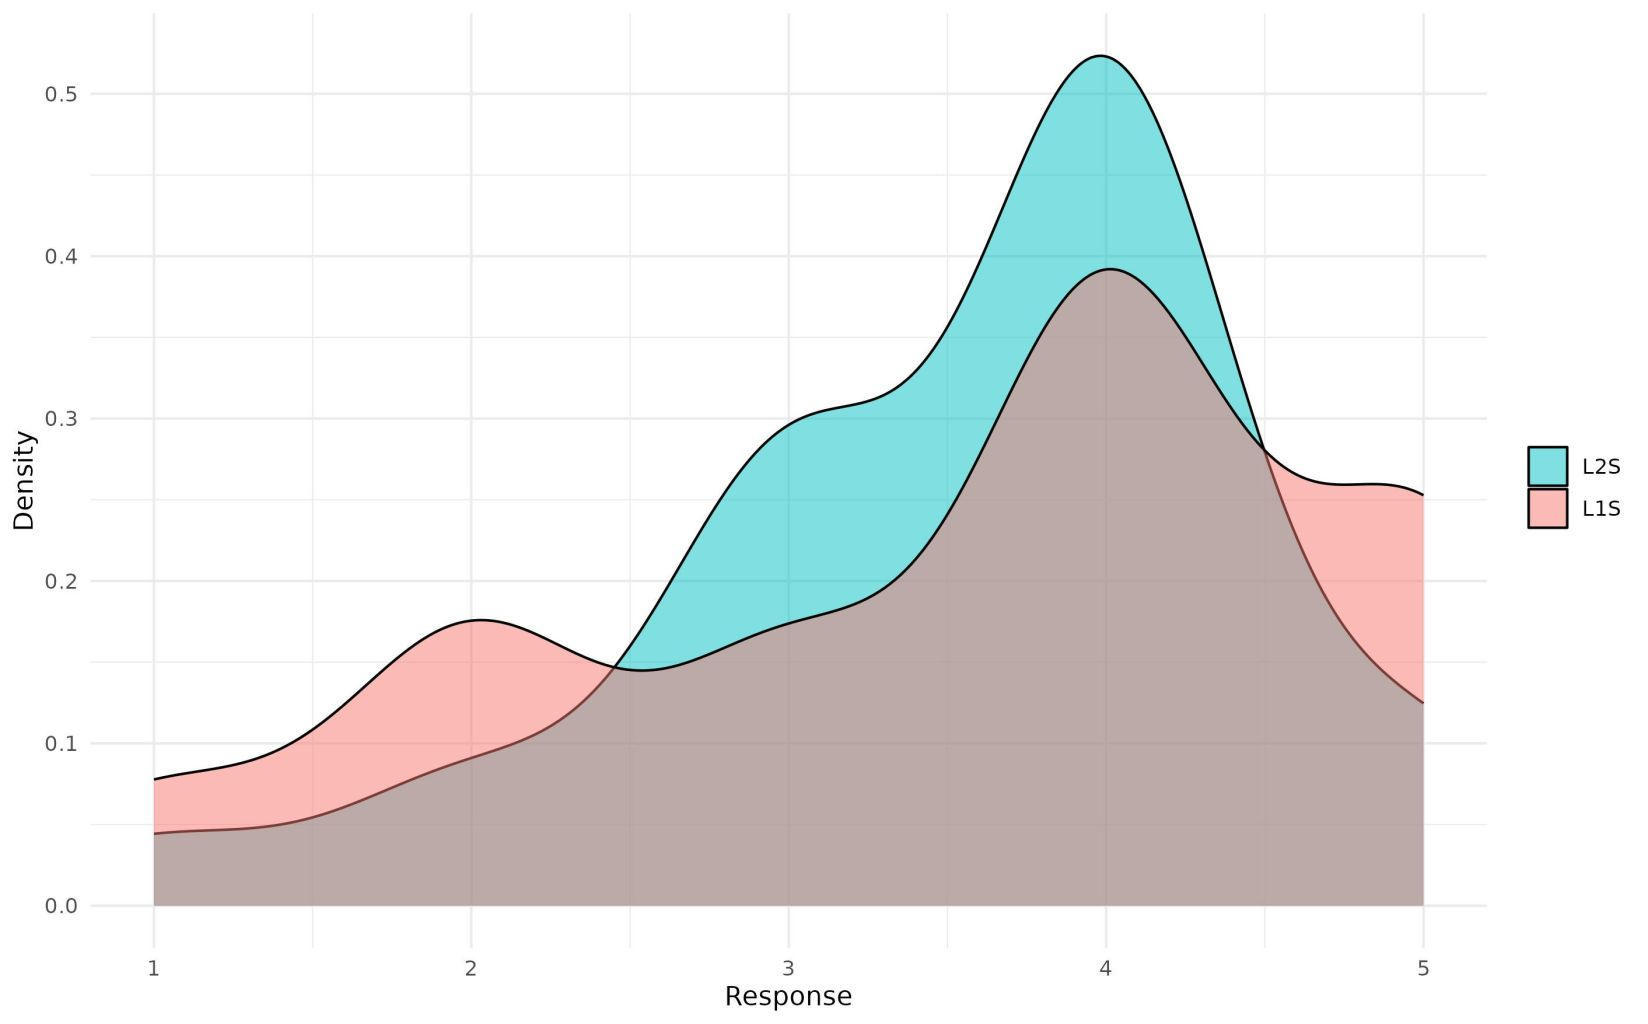
\includegraphics[width=\textwidth]{figures/Chapter4Ezeizabarrenaetalformatted-img001.jpg}
\caption{Distribution of the overall responses for mixed DPs per bilingual group. Note that the y-axis represents the probability density estimation, ranging from 0 to 1. This roughly translates into actual response percentages, a probability of 0.5 reflecting 50\% of responses.}
\label{fig:ezeiza:1}
\end{figure}

{In general, both bilingual groups seemed to behave quite similarly with regard to the acceptability rates, as indicated by the high mean and median scores (mean: 3.54/3.55 and median 4/4 for the L1S/L2S groups respectively). Moreover, similar intragroup variability was attested, as revealed by the wide range of scores <1-5> in both groups, and the standard deviation (1.22/0.92) respectively. In fact, some participants (2 L1S and 4 L2S participants) never selected the} {\textit{good}} {option in the scoring of mixed experimental sentences, which contrasts with their high scores for unilingual sentences (5 scores).}

{However, some differences appeared between the groups. As plotted in \figref{fig:ezeiza:1}, a primary peak at score 4 or} {\textit{strange but acceptable}} {option, and a secondary peak at score 2 or} {\textit{very strange,}} {evidenced a bimodal distribution in the L1S group’s responses, which revealed as a more polarized response pattern than the L2S group’s. The latter showed a centered/unimodal distribution with a single peak around score 3} {\textit{quite strange}} {and score 4} {\textit{strange but acceptable}}{, with higher frequencies than the L1S around these two values. As we will see, this} {difference is not statistically robust on its own, but it does interact with other factors.}

{Next, we compared the acceptability rates across conditions, in order to check differences between a(nalogical) or p(honological) gender assignment strategies (GAS). General acceptability rates appeared as less uniformly distributed when analysing data across conditions. The most accepted condition was condition a1-p1 \REF{ex:ezeiza:19a}, with acceptability rates over 68\% (}{\textit{acceptable}} {(49.09\%) plus} {\textit{good}} {(19.55\%)). In this condition there was a double match, as the gender feature of the determiner matched both the gender feature of the Spanish equivalent of the Basque noun (}{\textit{analogical match}} {or a1), and the phonological ending of the Basque noun (}{\textit{phonological match}} {or p1). Slightly lower acceptability rates were observed for the two match-mismatch conditions, with 64.09\% acceptance rate for the analogical mismatch-phonological match condition or a0-p1 \REF{ex:ezeiza:19b} and 62.73\% for the analogical match-phonological mismatch or a1-p0 condition \REF{ex:ezeiza:19c}, with a very small difference of 1\% between them. Finally, the double-mismatch a0-p0 condition \REF{ex:ezeiza:19d} was the worst rated, which obtained the} {\textit{acceptable}} {or} {\textit{good}} {rate from less than half of the participants (48.64\%). See \tabref{tab:ezeiza:4}.}

\ea\label{ex:ezeiza:19}
\ea\label{ex:ezeiza:19a}
a1-p1 \\ el      soineko

   the\textsubscript{M} dress (Spanish: vestido\textsubscript{M})

             ‘the dress’

\ex\label{ex:ezeiza:19b}
a0-p1   \\  la     gazta

 {the}{\textsubscript{F}} {cheese (Spanish: queso}{\textsubscript{M}})

                         ‘the cheese’

\ex\label{ex:ezeiza:19c}
a1-p0  \\  la      jostorratz

 {the}{\textsubscript{F} }{needle (Spanish: aguja}{\textsubscript{F}})

                          ‘the needle’

\ex\label{ex:ezeiza:19d}
a0-p0 \\   el       kaiola

 {the}{\textsubscript{M}} {cage (Spanish: jaula}{\textsubscript{F}})

                           ‘the cage’
\z
\z

\begin{table}
\small
\begin{tabularx}{\textwidth}{QrrrrrrrY}
\lsptoprule
{ Condition}  & \multicolumn{5}{c}{{ Responses (\%)}} & { Mean} & { SD} & { Acceptance (r4 +r5)}\\
\midrule
%\hhline%%replace by cmidrule{-~~~~~---} & { r1} & { r2} & { r3} & { r4} & { r5} &  &  & \\
{ a0-p0} & { 9.09} & { 18.18} & { 24.09} & { 37.73} & { 10.91} & { 3.24} & { 1.13} & { 48.64}\\
{ a1-p0} & { 5.00} & { 13.18} & { 18.64} & { 48.64} & { 14.09} & { 3.54} & { 1.05} & { 62.73}\\
{ a0-p1} & { 4.09} & { 9.55} & { 22.28} & { 40.91} & { 23.18} & { 3.70} & { 1.05} & { 64.09}\\
{ a1-p1} & { 4.09} & { 7.73} & { 19.09} & { 49.09} & { 19.55} & { 3.73} & { 0.99} & { 68.64}\\
\tablevspace
{ Analogical conditions}
{ a1-(p0 \& p1)}  & { 4.54} & { 10.45} & { 18.86} & { 48.9} & { 16.81} & { 3.635} &  & { 65.68}\\
\tablevspace
{ Phonological conditions}
{  (a0 \& a1)-p1} & { 4.09} & { 8.63} & { 20.68} & { 45} & { 21.4} & { 3.7125} &  & { 66.36}\\
\lspbottomrule
\end{tabularx}

\caption{Distribution of responses 1 to 5 by condition.}
\label{tab:ezeiza:4}
\end{table}

{Grouping the four conditions allowed the comparison of results by gender assignment strategies. No clear differences were observed between the analogical (a1-p0 and a1-p1) and the phonological conditions (a0-p1 and a1-p1), where frequencies of (clear) acceptance (}{\textit{acceptable}} {+} {\textit{good}} {responses) were almost the same for the analogical (a1p0 + a1p1) and the phonological ones (a0p0+a1p0), 65.68\% and 66.36\% respectively. See \tabref{tab:ezeiza:4}.}

{Overall, no major differences were observed between L1S and L2S groups either (mean 61\% in each group) for the two acceptance responses (4} {\textit{strange but}} {\textit{acceptable}} {and 5} {\textit{good}} {together). In contrast, rates of rejection varied: L1S group’s rejection rates (response 2} {\textit{very strange}} {and 1} {\textit{bad}} {together) were twice as big as L2S group’s, in general (24\% vs. 12\%), and for all the four conditions, as displayed in \figref{fig:ezeiza:2}. This resembles \figref{fig:ezeiza:1}, where L1S participants gave more polarized responses, by making greater use of the lower end of the scale than L2S participants).}

\begin{figure}
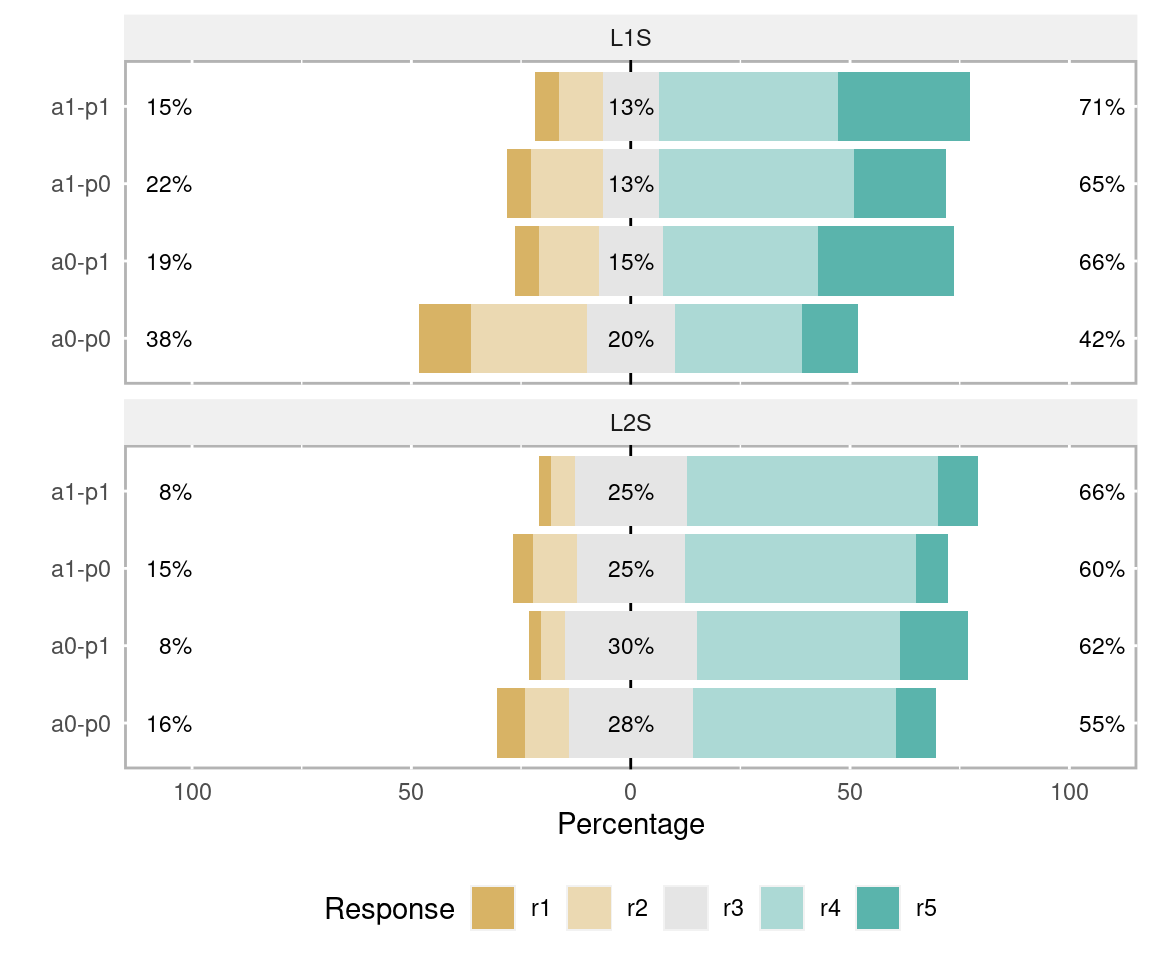
\includegraphics[width=\textwidth]{figures/Chapter4Ezeizabarrenaetalformatted-img002.png}
~
\caption{Distribution of responses (frequency) by condition and group}
\label{fig:ezeiza:2}
\end{figure}

{As shown in \figref{fig:ezeiza:2}, the following ranking of conditions can be identified, which appears as consistent across the three samples (total and both group samples): a1-p1 ${\geq}$ a0-p1${\geq}$ a1-p0 > a0-p0. This finding contrasts, however, with the similar acceptance frequencies obtained for the two analogical and phonological GAS in the whole sample. Figures \figref{fig:ezeiza:2} and \figref{fig:ezeiza:3b} indicate that the less uniform distribution of the L1S group’s responses extended across test conditions, except for a0-p0.}

{Taking group and conditions into account (\figref{fig:ezeiza:2}), the phonology matching conditions received the highest and similar scores from both groups, with a slight difference of 4-5\% between the groups, in both the additional analogical match a1-p1 (L1S/L2S 66/71\%) and the mismatch a0-p1 (L1S/L2S 66/62\%), followed by the a1-p0 condition (L1S/L2S 65/60\%). The two groups differed the most in the worst rated mismatch condition a0-p0 (L1S/L2S 42/55\%).}

{It is noteworthy that the L1S group showed a differentiated pattern for the three (single- or double-)matching conditions – both analogical and} {phonological match (a1-p1), only analogical (a1-p0) and only phonological match (a0-p1) – with high acceptance rates from 65\% to 71\%, as compared to the considerably lower acceptance rate (42\%) of non-matching items (a0-p0). In contrast, the L2S group showed a more homogeneous and moderately lower acceptance rate across the three matching conditions (60-66\%), and the lowest score in the mismatch condition (55\%) (\figref{fig:ezeiza:2}).}

{We performed a linear mixed model} {\citep{BatesEtAl2015}} {in order to analyse the effect as well as the interaction between the (four) experimental conditions and the two bilingual groups, L1S vs. L2S. Participant and item IDs were added as random factors to the model, in order to account for the non-independence of the responses.}

Model 1. \textit{response {\textasciitilde} condition * L1S + (1{\textbar}participant\_id) + (1{\textbar}item\_id)}

Model 1 revealed that experimental condition and group, taken separately, are not statistically significant predictors of judgment results (\tabref{tab:ezeiza:5}). L1S speakers showed overall lower scores, but this difference did not reach significance (\textit{t}=-1.51, \textit{p}=0.13). However, a noteworthy interaction arose between the two predictors (condition and bilingual group), in the sense that, compared to the L2S group, L1S speakers’ responses showed statistically significant differences between conditions. Taking condition a0-p0 as a baseline, where no analogical/phonological cue is satisfied, the L1S group judged all the other conditions significantly better, the strongest effect being under condition a1-p1 (\textit{t}=3.52, \textit{p}=<0.001), followed by a1-p0 (\textit{t}=3.07, \textit{p}=0.002) and a0-p1 (\textit{t}=2.69, \textit{p}=0.007). These effects can be visualized in \figref{fig:ezeiza:2}, where the L1S group gave a score of 4 or 5 to less than half (42\%) of the items in condition a0-p0. This rate differs from the higher rates of 4-5 scores (66-71\%) observed in the other three conditions. In contrast, the responses by L2S speakers were less polarized, and no significant differences were found between conditions.

\begin{table}
\begin{tabularx}{\textwidth}{Xrrrr}
\lsptoprule
  & \multicolumn{4}{c}{{ Score}}\\
{ \textit{Predictors}} & { \textit{Estimates}} & { \textit{CI}} & { \textit{t}} & { \textit{p}}\\
\midrule
{ (Intercept)} & { 3.43} & { 3.03~–~3.82} & { 17.05} & { <0.001***}\\
{ a0-p1} & { 0.24} & { {}-0.08~–~0.57} & { 1.49} & { 0.137}\\
{ a1-p0} & { 0.06} & { {}-0.26~–~0.38} & { 0.37} & { 0.709}\\
{ a1-p1} & { 0.21} & { {}-0.11~–~0.53} & { 1.28} & { 0.202}\\
{ L1S}  & { {}-0.39} & { {}-0.90~–~0.12} & { {}-1.51} & { 0.130}\\
{ a0-p1:L1S} & { 0.44} & { 0.12~–~0.76} & { 2.69} & { 0.007**}\\
{ a1-p0:L1S} & { 0.50} & { 0.18~–~0.82} & { 3.07} & { 0.002**}\\
{ a1-p1:L1S} & { 0.57} & { 0.25~–~0.89} & { 3.52} & { <0.001***}\\
{ n~\textsubscript{subj\_id}} & \multicolumn{4}{c}{{ 22}}\\
{ n~\textsubscript{item\_id}} & \multicolumn{4}{c}{{ 80}}\\
{ Observations} & \multicolumn{4}{c}{{ 878}}\\
{ Marginal R\textsuperscript{2}~/ Conditional R\textsuperscript{2}} & \multicolumn{4}{c}{{ 0.042 / 0.401}}\\
\lspbottomrule
\end{tabularx}
\caption{Results of Linear Mixed Model 1, testing the effect of experimental condition and bilingual group.}
\label{tab:ezeiza:5}
\end{table}

{We performed a second linear mixed model (Model 2), in order to analyse the effect as well as the interaction between the (four) experimental conditions, the M vs. F gender feature of the Spanish determiner, and the (two) bilingual Basque-Spanish groups, L1S  and L2S.}

Model 2: \textit{response {\textasciitilde} condition * det\_gender * L1+ (1{\textbar}participant\_id) + (1{\textbar}item\_id)}

Means and boxes plotted in \figref{fig:ezeiza:3}a indicate that acceptability rates for M vs. F differ in the range of <0.05-0.45> across conditions and groups. Here too, the L1S group (but not the L2S group) showed a differentiated pattern for matching (single- or double-) or cued and non-matching (uncued) conditions. Acceptability means were higher for M items than for F ones in the three cued conditions, where the mean differences in acceptability of M items ranged <0.08-0.45> across conditions, whereas F items scored over M in the non-matching condition a0-p0 (0.61). This suggests that the difference between a0-p0 (\ref{ex:ezeiza:20a}a,b) and the other conditions observed in \figref{fig:ezeiza:2} and \tabref{tab:ezeiza:5} is mainly driven by the rejection of M Det\textsubscript{S} preceding –\textit{a} ending N\textsubscript{B} under a0-p0 \REF{ex:ezeiza:20b}. See also \figref{fig:ezeiza:3}b.

\ea \label{ex:ezeiza:20a}
\ea  a0-p0 \\  la     soineko

 {the}{\textsubscript{F}} {dress (Spanish: vestido}{\textsubscript{M}})

 {‘the dress’}
\ex \label{ex:ezeiza:20b} a0-p0  \\  el      kaiola

      the\textsubscript{M}  cage (Spanish: jaula\textsubscript{F})

{‘the cage’}

\z
\z

In contrast, the L2S group showed a pattern where F items were scored higher than M, in the non-matching a0-p0 condition (0.13 difference) but also in the two single matching conditions, namely a1-p0 (0.09) and a0-p1 (0.26). There is one only condition in which M is scored over F, though very slightly: a1-p1 (0.06).

\begin{figure}
\subfigure[Mean acceptability rates by group, condition and gender of DetS\label{fig:ezeiza:3a}]{
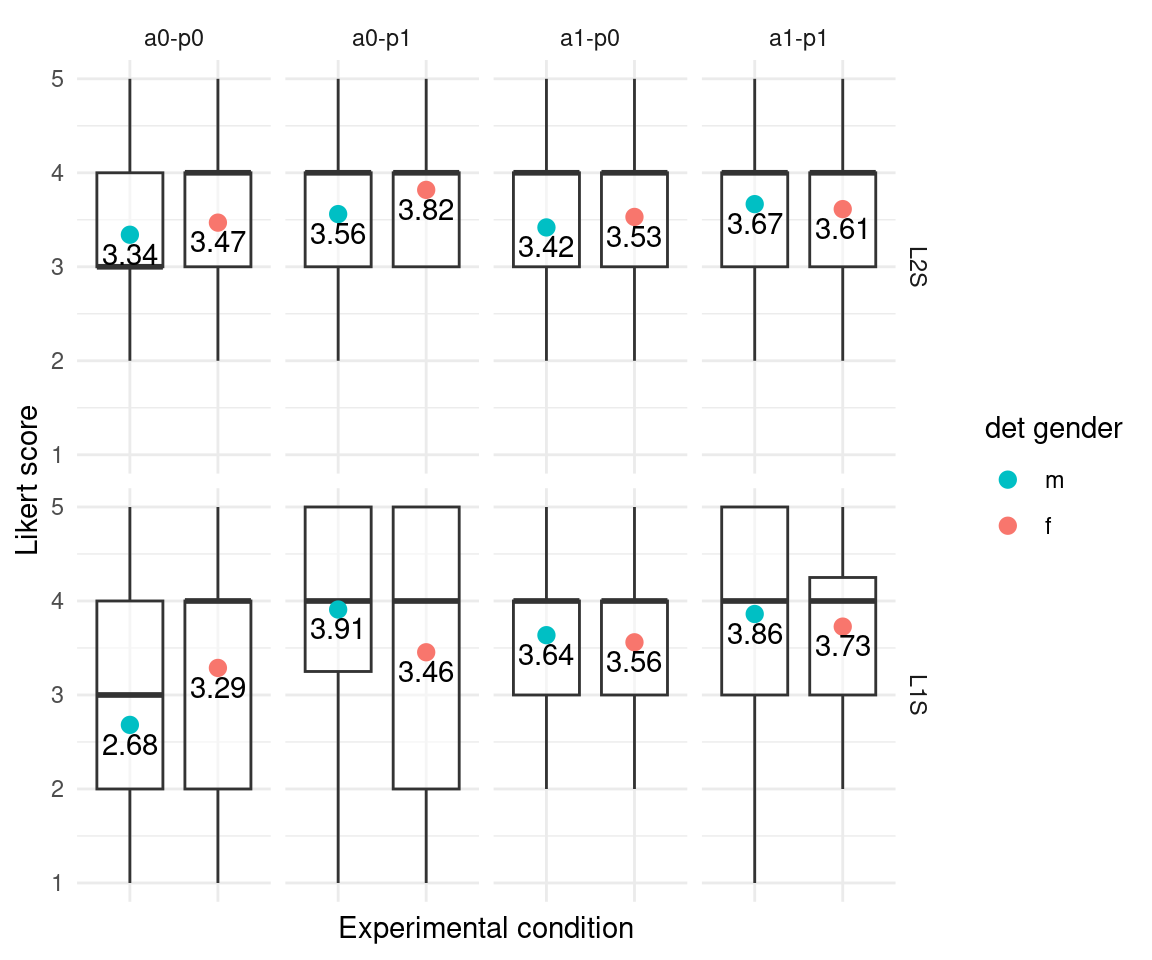
\includegraphics[width=.9\textwidth]{figures/Chapter4Ezeizabarrenaetalformatted-img003.png}
}
\subfigure[Density plot illustrating responses by group, condition and gender of the determiner\label{fig:ezeiza:3b}]{
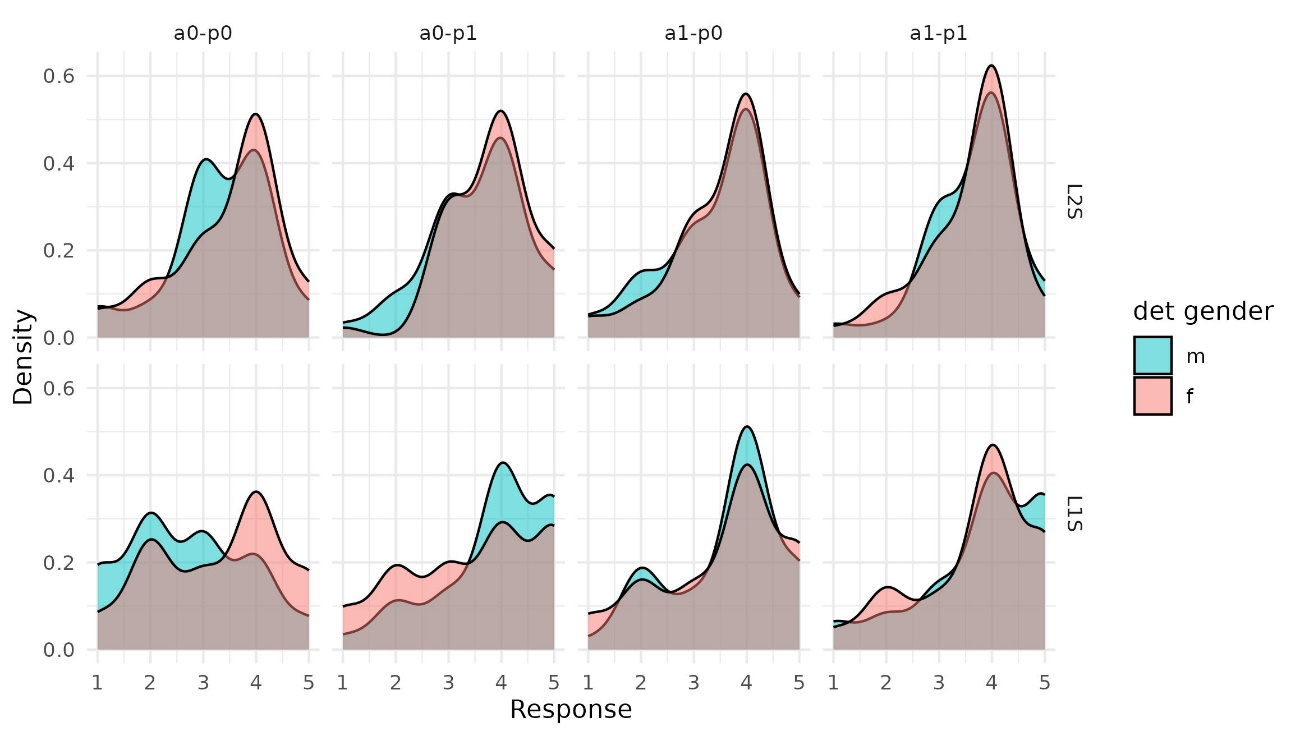
\includegraphics[width=.9\textwidth]{figures/Chapter4Ezeizabarrenaetalformatted-img004.jpg}
}
\caption{Group, condition, and gender}
\label{fig:ezeiza:3}
\end{figure}

Taking a0-p0 condition and L2S as baseline, Model 2 revealed that gender (\textit{t}= 0.53; \textit{p}=0.594) taken separately is not a statistically significant predictor of the judgment results (see \tabref{tab:ezeiza:6}). Nevertheless, group (t=-2.32; p=0.021) as well as the interaction of group and condition (p<0.001), and group and gender (t=2.06; p=0.039) revealed significant. A three-way interaction between group, condition and gender can be observed in the rejection of M items by the L1S group under the a0-p0 non-matching condition \REF{ex:ezeiza:20b} plotted in Figures \figref{fig:ezeiza:3a} and \figref{fig:ezeiza:3b}.

\begin{table}
\begin{tabularx}{\textwidth}{Xrrrr}
\lsptoprule
{  } & \multicolumn{4}{c}{{ Score}}\\
{ \textit{Predictors}} & { \textit{Estimates}} & { \textit{CI}} & { \textit{t}} & { \textit{p}}\\
\midrule
  (Intercept)  &   3.35 \textsuperscript{***}   &   2.87 – 3.84  &   13.59  &   <0.001 \\
 Condition 0-1 &  0.21 &  -0.25 – 0.68 &  0.89 &  0.371\\
 Condition 1-0 &  0.08 &  -0.44 – 0.59 &  0.30 &  0.766\\
 Condition 1-1 &  0.30 &  -0.16 – 0.77 &  1.28 &  0.202\\
 art gender [f] &  0.13 &  -0.34 – 0.59 &  0.53 &  0.594\\
  L1S [1]  &     -0.68 \textsuperscript{*}   &     -1.26 – -0.10  &     -2.32  &   0.021 \\
 Condition 0-1: art [f] &  0.14 &  -0.52 – 0.80 &  0.43 &  0.670\\
 Condition 1-0: art [f] &  -0.03 &  -0.69 – 0.63 &  -0.08 &  0.934\\
 Condition 1-1: art [f] &  -0.17 &  -0.83 – 0.49 &  -0.51 &  0.607\\
  Condition 0-1: L1S  &   1.02 \textsuperscript{***}   &   0.56 – 1.48  &   4.38  &   <0.001 \\
  Condition 1-0: L1S  &   0.90 \textsuperscript{***}   &   0.40 – 1.41  &   3.52  &   <0.001 \\
  Condition 1-1: L1S  &   0.90 \textsuperscript{***}   &   0.44 – 1.36  &   3.87  &   <0.001 \\
  art [f] × L1S [1]  &   0.48 \textsuperscript{*}   &   0.02 – 0.94  &   2.06  &   0.039 \\
  Condition 0-1: art [f]: L1S  &     -1.22 \textsuperscript{***}   &     -1.87 – -0.57  &     -3.70  &   <0.001 \\
  Condition 1-0: art [f]: L1S  &     -0.67 \textsuperscript{*  } &     -1.32 – -0.02  &     -2.02  &   0.043 \\
  Condition 1-1: art [f]: L1S  &     -0.58  &     -1.23 – 0.07  &     -1.76  &   0.078 \\
{ n \textsubscript{subj\_id}} & \multicolumn{4}{c}{{ 22}}\\
{ n \textsubscript{item\_id}} & \multicolumn{4}{c}{{ 80}}\\
{ Observations} & \multicolumn{4}{c}{{ 878}}\\
{ Marginal R\textsuperscript{2} / Conditional R\textsuperscript{2}} & \multicolumn{4}{c}{{ 0.059 / 0.417}}\\
\multicolumn{5}{c}{{ \textit{p<0.05   ** p<0.01   *** p<0.001}}}\\
\lspbottomrule
\end{tabularx}

\caption{Results of Linear Mixed Model 2, testing the effect of experimental condition, gender of DetS, and bilingual group.}
\label{tab:ezeiza:6}
\end{table}

{Finally, we performed a third linear mixed model (Model 3), in order to analyse the effect of the type of} {\textit{-a}} {ending (lexical vs. grammatical) on a subset of 88 items.}

Model 3: \textit{response {\textasciitilde} word ending * L1 + (1{\textbar}participant\_id) + (1{\textbar}item\_id)}

{The mixed regression revealed that neither word ending (lexical vs. grammatical) nor the interaction between word ending and bilingual group reached significance (\tabref{tab:ezeiza:7}). In other words, the lexical (a1-p1} {\textit{la tipula} }{‘the onion’, a0-p1} {\textit{la zozketa} }{‘the raffle’) vs. grammatical nature (a1-p1} {\textit{la etxe-a} }{‘the house’, a0-p1} {\textit{la soineko-a} }{‘the dress’) of the} {\textit{-a}} {ending in Basque added to the root of the inserted N}{\textsubscript{B}} {has no effect on the acceptability of the mixed DPs. Nevertheless, the different curves obtained for the two groups in the analogical mismatch conditions (a0-p0 and a0-p1) will require further research (\figref{fig:ezeiza:4}).}

\begin{figure}
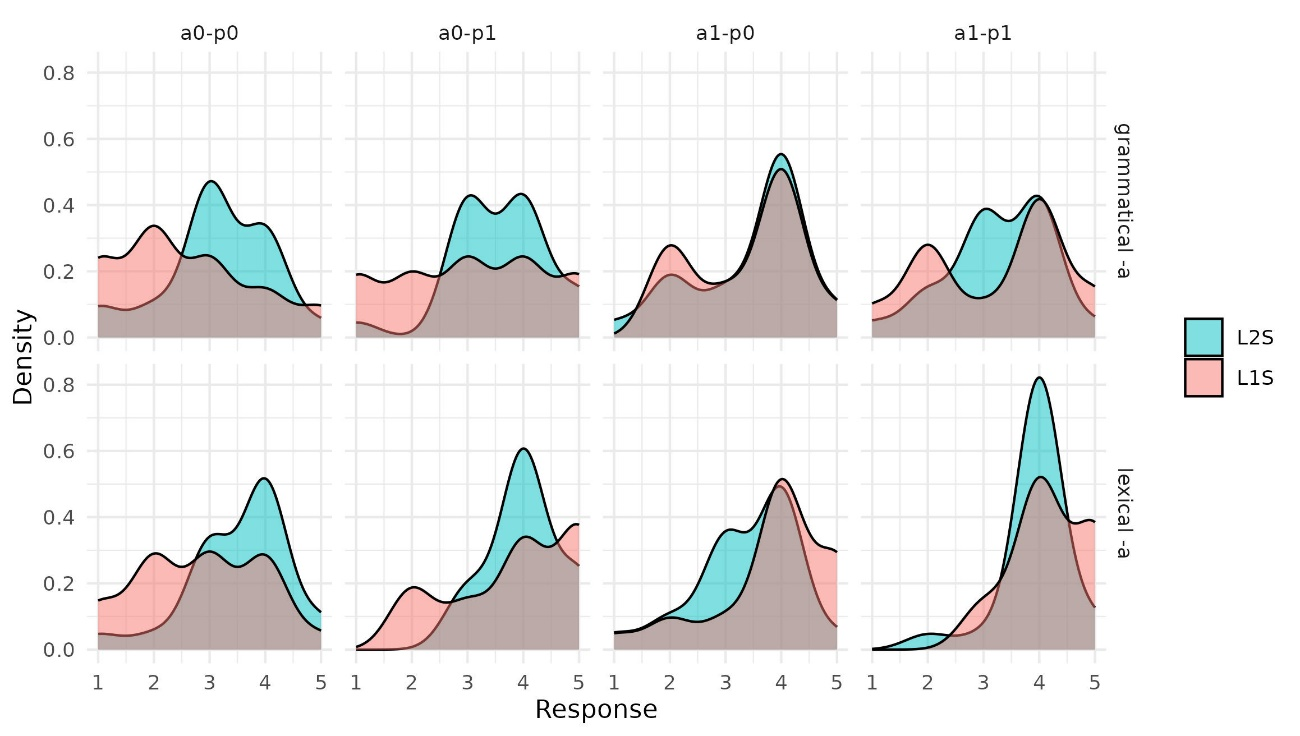
\includegraphics[width=\textwidth]{figures/Chapter4Ezeizabarrenaetalformatted-img005.jpg}
\caption{Density plot illustrating the acceptance responses of mixed DPs with lexical -a vs. grammatical -a, by bilingual group in four conditions.}
\label{fig:ezeiza:4}
\end{figure}

\begin{table}
\begin{tabularx}{\textwidth}{Xrrrr}
\lsptoprule
{  } & \multicolumn{4}{c}{{ Response}}\\
{ \textit{Predictors}} & { \textit{Estimates}} & { \textit{CI}} & { \textit{Statistic}} & { \textit{p}}\\
\midrule
 (Intercept) &  4.06 \textsuperscript{***} &  3.40 – 4.71 &  12.29 &  <0.001\\
 word end [2] &  --0.44 &  --1.27 – 0.39 &  --1.05 &  0.298\\
 spaL1 [L1S] &  --0.20 &  --0.85 – 0.45 &  --0.62 &  0.535\\
 word end [2] × spaL1 [L1S] &  --0.40 &  --1.11 – 0.31 &  --1.12 &  0.266\\
{ n \textsubscript{subj\_id}} & \multicolumn{4}{c}{{ 22}}\\
{ n \textsubscript{item\_id}} & \multicolumn{4}{c}{{ 8}}\\
{ Observations} & \multicolumn{4}{c}{{ 88}}\\
{ Marginal R\textsuperscript{2} / Conditional R\textsuperscript{2}} & \multicolumn{4}{c}{{ 0.118 / 0.471}}\\
\multicolumn{5}{c}{{ \textit{p<0.05   ** p<0.01   *** p<0.001}}}\\
\lspbottomrule
\end{tabularx}
\caption{Results of Linear Mixed Model 3, testing the effect of {\textit{-a}} word ending (grammatical or lexical) and bilingual group.}
\label{tab:ezeiza:7}
\end{table}

\section{Discussion and conclusions}\label{sec:ezeiza:5}

The two groups of Basque-Spanish bilinguals tested with an acceptability task evidenced a very heterogeneous acceptance pattern for mixed sentences containing a Det\textsubscript{S}N\textsubscript{B}, where rates oscillated along the whole score range of 1 to 5. In contrast, they showed a consistent acceptance (rated as 5) of both unilingual Spanish and Basque sentences.

The low frequency of low scores (1. \textit{bad} and 2. \textit{very strange} combined (<20\% together) and the considerably high mean (3.548) and median (4) values in the total sample for both L1S and L2S groups, suggests that the participants tested are familiar with mixed DPs, generally accept them, and that Det\textsubscript{S}N\textsubscript{B} structures in particular are part of the speech of their community.

Noticeably, 5. \textit{good} responses were scarce and 27\% of the participants (2 L1S and 4 L2S) did not select that option when judging experimental (mixed) items, which indicates that the bilinguals tested considered Det\textsubscript{S}N\textsubscript{B} structures \textit{strange} or even \textit{bad} (score 1) rather than normal, as shown by the frequency of 2-4 scores (2. \textit{very strange}, 3. \textit{quite strange}, 4.  \textit{strange but acceptable}). This pattern was found in both L1S and L2S groups. The individual variation attested is in line with the variation found in previous research, which tested some “conflict sites” (\citealt{PoplackMeechan1998}) in elicited and/or spontaneous production (\citealt{Cruz2023,DuBord2004,OthegyLapidus2003,PoplackEtAl1982}), but also in the acceptability of mixed sentences involving language switch in structures involving Det\textsubscript{S}{}-N\textsubscript{Language X} structures (\citealt{Beatty-MartínezDussias2019,BellamyParafitaCouto2022,LicerasFernándezFuertes2018,LicerasEtAl2008,ValdésKroffEtAl2017}).

Unlike the bilinguals tested in the use of mixed DPs involving Det\textsubscript{S}N\textsubscript{B} \citep{Munarriz-IbarrolaEtAl2022}, the bilinguals tested in the current study did not show any clear preference for M or F mixed DPs. This contrasts with previous production and acceptance studies reporting M preference (\citealt{BadiolaSande2018,Cruz2023,ValdésKroff2016,ValdésKroffEtAl2017}), or F preference (\citealt{ParafitaCoutoEtAl2015basque}) for DetS preceding lexical insertions (N) from ungendered languages. By group, the L1S showed higher mean scores for M in the cued conditions, whilst an F preference was found in the non-matching (uncued) condition. In fact, either equal or very slightly higher mean scores for F were attested across conditions in the L2S group. The Linear Mixed Model 2, which included gender, bilingual group and response conditions, revealed no significant differences except for the a0-p0 condition in the L1S group, where F mixed DPs obtained significantly higher scores than M. Far from confirming the M default strategy, according to which Det\textsubscript{S} in mixed DPs are predominantly M (\citealt{Beatty-MartínezDussias2019,ValdésKroff2016}), the current findings on Det\textsubscript{S}N\textsubscript{B} are more compatible with a constraint default strategy, which is restricted to a) a particular type of words (that is, in uncued or non-matching conditions), rather than extensible to all nouns, or to broad semantic categories such as inanimate nouns, in line with \citet{Munarriz-IbarrolaEtAl2022} but in contrast to \citet{Cruz2023}; and to b) specific bilingual profiles (non-Spanish dominant) in line with \citet{LicerasEtAl2008} and  \citet{LicerasFernandezFuertes2018}, rather than to specific communities defined in geographical or specific language-contact situations.

In line with prediction 1, sentences with Det\textsubscript{S}N\textsubscript{B} structures did not show the same acceptance or rejection pattern across the four experimental conditions of a(nalogical) match (1) / mismatch (0) and p(honological) match (1) /mismatch (0): a1-p1, a1-p0, a0-p1 and a0-p0. The double-matched a1-p1 condition obtained the highest mean scores, followed by single-matching a0-p1 and a1-p0 conditions, and then by the non-matched a0-p0 condition, which obtained the lowest scores. This general pattern was attested in the total as well as in the two group samples, L1S and L2S.

The second prediction of higher acceptability rates for the phonological matching conditions (a0-p1 \textit{la basoa, el gorringo} and a1-p1 \textit{la ezkontza}, \textit{el soineko}) than for the phonological mismatch conditions (a1-p0 \textit{la gorringo}, \textit{el basoa} and a0-p0 \textit{el etxea}, \textit{la soineko}) has been only partially confirmed, since total mean scores for a0-p1 and a1-p1 conditions were higher than for a0-p0. However, they were not notably higher than a1-p0 in both groups. The similar mean scores obtained in the analogical matching conditions (a1-p1 and a1-p0 combined) and the phonological matching conditions (a0-p1 and a1-p1 combined) discard the exclusion of either GAS: the phonological strategy (Prediction 2, \citealt{Harris1991,TeschnerRussell1984}) and the analogical strategy (Prediction 4). Rather than a competition, the high mean scores of the double matching condition suggests a summative compatibility of the two GAS (prediction 5). However, differences in mean scores found among the three cued conditions (a1-p1, a1-po and a0-p1) in the whole sample did not reach statistical significance. Statistical differences were found between the non-matching a0-p0 and the other three conditions, but only for the L1S group, where despite the small sample of 11 participants, the two analogical matching conditions (both a1-p1 and a1-p0) obtained the highest acceptability scores, followed by the only phonological matching condition (a0-p1) confirming predictions 5 and 6. The L2S group, equally small, provided data that did not reach statistical significance. Nevertheless, the acceptability pattern of L2S appeared as compatible with the prediction of a phonological GAS preference, where the doubly matching a1-p1 condition obtained the highest mean scores, followed by the phonological matching condition (a0-p1). Nevertheless, the analogical GAS is also active in this group, as shown by the closeness of the mean scores obtained in the preceding and the a1-p0 condition. Both groups' preferences seem to be aligned – although at different strength – with the analogical GAS or the “correct gender agreement” \citep{JorschickEtAl2011}. Additional evidence for the analogical strategy over the masculine default in mixed DPs involving Spanish has been provided by \citet{LicerasFernándezFuertes2018,LicerasFernándezFuertessubmitted} in Spanish-English mixed DPs, across bilingual populations of Spanish-English bilinguals from Trinidad and Tobago (bilingual children with English vs. Spanish as heritage language, L2S speakers with advanced vs. intermediate level). Despite the differences found across tasks (acceptance, sentence completion), the higher acceptance of analogical match in mixed English-Spanish DPs for advanced than for less advanced L2S learners is in line with the assumption that variation in GAS is generally modulated by bilingual profile, and that the preference for the analogical strategy in Spanish-speaking bilinguals in particular may be associated with a higher level of competence or frequency of use of Spanish than of the ungendered language (B or E). See also \citet{ValdésKroffEtAl2017}.

The third prediction regarding the contrast between two types of \textit{-a} endings seems not to be confirmed either, since participants did not show any preference for DPs with F Det preceding nouns with lexical \textit{{}-a} endings, as compared to Basque nouns with the grammatical suffix article \textit{-a}. Contrary to \citet{BadiolaSande2018}, participants in the current study did not score F items such as a1-p1 \textit{la ezkontza} ‘wedding’ or a0-p1 \textit{la zozketa} ‘lottery’ higher than F a1-p1 \textit{la etxe-a} ‘house-the’, a0-p1 \textit{la ogi-a} ‘bread-the’ with grammatical \textit{-a} ending. The mixed regression analyses did not reveal significant differences in this regard. The current findings are more in line with the acceptability results of \citet{ParafitaCoutoEtAl2015basque} and the production data by \citet{Munarriz-IbarrolaEtAl2022}, who concluded that cued GAS rather than default strategies could account for the variability attested. For instance, some participants (A7, A8, B8) showed more intraindividual variation than others by alternating in the form of the lexical insertion N\textsubscript{B} in the mixed DP: (A7\textit{: el eztia} a0-p0\textit{, el ezti} a0-p1 ‘the\textsubscript{M} honey\textsubscript{F}’; B8: \textit{la eguzkia} a0-p1\textit{, la eguzki} a0-p0 ‘the\textsubscript{F} sun\textsubscript{F}’; A8: \textit{la eztia} a1-p1\textit{, la ezti} a1-p0 ‘the\textsubscript{F} honey\textsubscript{F}’). Interestingly, gender was found to vary interindividually \textit{el/la ezti(a)} in those alternating pairs, but it was the form of the nominal insertion, \textit{ezti} (root) vs. \textit{eztia} (root + \textit{{}-a} ending), rather than Det\textsubscript{S} that showed intraindividual variation. These alternation patterns are in line with a quite stable individual representation of gender specificity as compared to the less stable representation of the form of the nominal insertion, according to which the Basque equivalent \textit{eztia} of the Spanish noun \textit{miel\textsubscript{F}} \textit{‘}honey’ may be assigned only one gender option (M by some bilinguals, F by others), but may vary in the form used by the same bilingual speaker when inserting it in mixed DPs: sometimes as a bare root (\textit{ezti}) and others as a morphologically complex word (\textit{ezti-a}).

All these findings are compatible with the first prediction that both rules, the compulsoriness  of gender assignment to Basque nouns and of the overt Det-N agreement,  also called “concord” (\citealt{LicerasFernándezFuertes2018}) are active in functional bilinguals’ (productive and evaluative) use of Det\textsubscript{S}N\textsubscript{B} structures. They also point towards the conclusion that both the analogical and the phonological GAS drive the Basque-Spanish bilinguals’ acceptance as well as the production of mixed DPs.  The different response patterns found in the acceptability task, according to which the L1S group appears as more sensitive than the L2S group to the cued/uncued distinction, as well as more analogically driven, support the claim that the strength or the hierarchy of GAS may be modulated by the bilingual profile (\citealt{LicerasEtAl2008,Munarriz-IbarrolaEtAl2022,ValdésKroffEtAl2017}).

Production and acceptability judgment data use seem to differ, in the strength of the specific GAS associated with the experimental conditions. The different GAS appear more clearly ranked for each group in production than in the acceptability judgments: analogical GAS as predominant for L1S vs. phonological GAS for L2S. The apparently contradictory results found in the two modalities of language use in Basque-Spanish mixed DPs are not an exception. Different GAS have also been identified in the production and acceptability judgment on mixed DPs by Spanish-Purepecha bilinguals. See \citet{BellamyEtAl2018} and    \citet{BellamyParafitaCouto2022}. In fact, different areas of the brain associated to executive functions such as the Anterior Cingular Cortex and the Dorsolateral Prefrontal Cortex) are involved in comprehension and production (\citealt{Blanco-ElorrietaPylkkänen2018}). Moreover, the linearity of online spontaneous and even elicited oral speech, as compared to the less linear parsing and (offline) processing involved in acceptability judgment tasks, may predict the different factors affecting production and acceptability of mixed DPs (differently). Note, for instance, that retrieving two words simultaneously in different languages (acceptability) is less cognitively demanding than having to inhibit the production of one, the dominant language \citep{Blanco-ElorrietaEtAl2018}.

In summary, the current acceptability data of mixed Det\textsubscript{S}N\textsubscript{B} structures by 22 Spanish-Basque bilinguals evidences that acceptability judgments on mixed DPs are driven by cued strategies, rather than by default ones. The present experiment, which was designed with the specific purpose of distinguishing the potential effects of the analogical and the phonological cues, has demonstrated that Basque-Spanish bilinguals, particularly those who demonstrate high competence in both languages, rely on both the analogical and the phonological GAS, and in a summative manner in the acceptability task.

We are aware of the limitations of the current study, and that more research with a bigger sample is required in order to support the results in a more conclusive way. Nevertheless, the present findings provide further corroboration for bilinguals' profile exerting an effect on their GAS and use of mixed DPs (\citealt{BellamyParafitaCouto2022,LicerasFernándezFuertessubmitted,ValdésKroffEtAl2017}).

\section*{Acknowledgments}

We want to express our gratitude to the people and institutions who made this research possible. First, we are grateful to the participants who volunteered in the data sampling, and to Alejandra Iriondo for her relevant collaboration in the preparation of the materials and in the data collection, as well as to the Basque Government (IT-1627-22) and the Ministry of Science, Innovation and University (PID2023-148030NB-I00), which supported the ELEBILAB research group.

\section*{Abbreviations}
\begin{tabularx}{.45\textwidth}{lQ}
 CS  &  Code Switching\\
 DP  &  Determiner Phrase\\
 N  &  Noun\\
 Det  &  Determiner\\
 Det\textsubscript{S}  &  Spanish Determiner\\
 Det\textsubscript{E}  &  English Determiner\\
 n  &  number\\
 N\textsubscript{E}  &  English Noun\\
 N\textsubscript{S}  &  Spanish Noun\\
 N\textsubscript{B}  &  Basque Noun\\
 E  &  English\\
 S  &  Spanish\\
 B  &  Basque\\
 \end{tabularx}
\begin{tabularx}{.45\textwidth}{lQ}
 F  &  Feminine\\
 M  &  Masculine\\
 PL  &  plural\\
 GAS  &  Gender Assignment Strategies\\
 RQ  &  Research Question\\
 L1  &  First Language\\
 L2  &  Second Language\\
 C1  &  Proficiency Qualification\\
 a0  &  analogical mismatch\\
 a1  &  analogical match\\
 p0  &  phonological mismatch\\
 p1  &  phonological match\\
 r  &  response
\end{tabularx}

\sloppy\printbibliography[heading=subbibliography,notkeyword=this]
\end{document} 
